% =====================================================================
% results.tex — section header + per-claim subsection stubs.
%
% Each subsection is filled by its own manuscript increment:
%   RB-009 -> sec:results-c1   (C1 distributional CF)
%   RB-010 -> sec:results-c2   (C2 + closed-form r†(v))
%   RB-011 -> sec:results-c3   (C3 graded regime, §5.2 design advice)
%   RB-012 -> sec:results-c4   (C4 conditional theorem + anti-cue)
%   (A1 lever sign-flip lives inside sec:results-c1 and sec:results-c2
%    rather than a dedicated A1 subsection, per the "three levers"
%    reframe in sec:model.)
%
% Allowed-strength ceiling: see CLAIM_LEDGER.md row by row.
% =====================================================================

\section{Results}
\label{sec:results}

The results are organised around the four headline claims of the
inherited paper, each restated at the strength licensed by the live
verdict ledger (\texttt{CLAIM\_LEDGER.md}). Section~\ref{sec:results-c1}
treats the criterion-fraction result (C1) as a \emph{distribution}
across the parameter sweep, not as a categorical floor.
Section~\ref{sec:results-c2}, the present subsection, treats the
non-monotonicity of VDA in the benefit/cost ratio $\Rsens$ (C2) as the
rebuild's \emph{confident spine}: a result that survives every attack
the skeptical reviewer has staged and that we strengthen here by
publishing a closed-form expression for the VDA-escape threshold
$\rdagger(\val)$ together with its empirical confirmation across a
$\val$-family. Section~\ref{sec:results-c3} reports the
regime-of-relevance (C3) as a graded boundary, replacing the original
``regardless of other parameters'' wording with a quantitative
iso-VDA band. Section~\ref{sec:results-c4} states the no-inversion
claim (C4) as a conditional theorem with the explicit condition
$\valid \ge 1/\Nloc$ and a new anti-cue corollary. Throughout, the
A1 decorrelation channel $\corr \in [0, 1)$
(Section~\ref{sec:model}) is reported \emph{alongside} each headline
result as a sensitivity, not segregated into its own subsection:
this is the operational meaning of the ``three levers, not two''
reframe.

% ---------------------------------------------------------------------
\subsection{Criterion fraction: distributional, not categorical (C1)}
\label{sec:results-c1}

\paragraph{Claim restated at defensible strength.}
The inherited paper introduces the \emph{criterion fraction}
%
\begin{equation}
  \CF \;:=\;
  \frac{\Rpfour - \Rew_{\text{baseline}}}{\Rpone - \Rew_{\text{baseline}}}
  \;=\;
  \frac{\text{criterion-only reward gain}}{\text{joint criterion + attention reward gain}}
  \label{eq:cf-def}
\end{equation}
%
as a one-number summary of how much of the optimal value-conditioned
reward gain can already be captured by re-aiming the per-location
decision criterion alone --- in the Müller--Findlay
\cite{MullerFindlay1987} sensitivity-vs-criterion vocabulary, the
``criterion shift'' lever --- with the residual $1 - \CF$ apportioned
to attention re-allocation. The inherited paper's headline summary of
this quantity (\texttt{Critique/source/main.pdf}, §5) is
\textbf{categorical}: $\CF$ is reported to lie in the interval
$[0.60, 0.96]$ across the primary $4{,}410$-cell
$(\Rsens, \valid, \val)$ sweep. The live skeptical-reviewer verdict
for this claim (\texttt{Critique/verdicts/C1--criterion-fraction-floor.md},
\texttt{current\_label: CONTESTED}) records that the true range is
$[0.30,\,1.00]$, and that the substantive ``criterion typically
dominates'' reading is sustained at the median but the categorical
floor is false at both ends. The rebuilt C1 therefore is presented in
this section as a \emph{distributional / central-tendency} result:
the full CF distribution is reported (range, median, quantiles, and
the fractions below $0.5$, $0.6$, $0.8$), and the headline statement
is downgraded from a categorical floor to a quantified central
tendency with explicit corner regions in which the criterion lever
becomes subordinate. The A1 decorrelation channel $\corr$ is
reported alongside the criterion-fraction distribution as a
sensitivity --- the convention established in
Section~\ref{sec:results} that operationalises the three-levers
reframe of Section~\ref{sec:model}.

\paragraph{Distribution across the primary 4{,}410-cell sweep.}
The primary sweep evaluates the rebuilt model at the headline
$\Nloc = 4$, $\dprimemax = 2$, $f_0 = 0.5$, $h = \sqrt{\;\cdot\;}$
configuration of Table~\ref{tab:r-dagger-family} on a grid of
$\valid \in [0.25, 1.00]$ ($21$ uniform points),
$\Rsens \in [0.1, 10]$ ($21$ log-spaced points), and $\val \in
\{1, 2, 3, 4, 5\}$, under both conservation variants (variant A:
$\benefit + \cost = 2$; variant B: $\benefit \cdot \cost = 1$), for
a total of $21 \times 21 \times 5 \times 2 = 4{,}410$
$(r,V,v)$-cells per variant. The full per-variant CF distribution at
$\corr = 0$ (the inherited independent model) is summarised in
Table~\ref{tab:cf-distribution}.
%
\begin{table}[t]
  \centering
  \small
  \begin{tabular}{l c c c c c c c c}
    \toprule
    variant & $\CF_{\min}$ & $q_{5\%}$ & $q_{25\%}$ & median &
    $q_{75\%}$ & $q_{95\%}$ & $\CF_{\max}$ & mean $\pm$ s.d.\\
    \midrule
    A & $0.5587$ & $0.5931$ & $0.6530$ & $\mathbf{0.7552}$
      & $0.8996$ & $1.0000$ & $1.0000$
      & $0.7773 \pm 0.1363$\\
    B & $\mathbf{0.3040}$ & $0.4564$ & $0.6288$ & $\mathbf{0.7682}$
      & $0.9463$ & $1.0000$ & $1.0000$
      & $0.7691 \pm 0.1808$\\
    \bottomrule
  \end{tabular}
  \caption{Distribution of the criterion fraction $\CF$ across the
  primary $4{,}410$-cell $(\Rsens, \valid, \val)$ sweep at the
  headline cell $(\Nloc, \dprimemax, f_0, h) =
  (4,\, 2,\, 0.5,\, \sqrt{}\,)$ under the inherited
  independence assumption $\corr = 0$, per conservation variant.
  Quantiles are over the $n = 2{,}205$ valid cells per variant.
  The inherited paper reports $\CF \in [0.60, 0.96]$; the true
  range is wider on both ends. Values from
  \texttt{Rebuild/sims/C1--cf-distribution/output/results.json}
  (rb-003; output sha256 \texttt{91fc4692\ldots}), block
  \texttt{summaries.variant\_A/rho\_0.0} and
  \texttt{summaries.variant\_B/rho\_0.0}.}
  \label{tab:cf-distribution}
\end{table}
%
Two things are visible. First, the \emph{central tendency} of the
inherited paper's reading survives intact: the median CF is
$0.7552$ in variant~A and $0.7682$ in variant~B, well above $0.5$
and consistent with the inherited paper's qualitative ``criterion
typically dominates'' framing. Second, the \emph{categorical floor}
fails at both ends: variant~A's strict minimum is $0.5587$ (below
the stated $0.60$) and variant~B's strict minimum is $0.3040$
(below $0.50$), while both variants achieve $\CF = 1.0$ in cells the
paper's stated upper bound of $0.96$ excludes. The full per-cell
histogram is given in Figure~\ref{fig:cf-histogram}.

\begin{figure}[t]
  \centering
  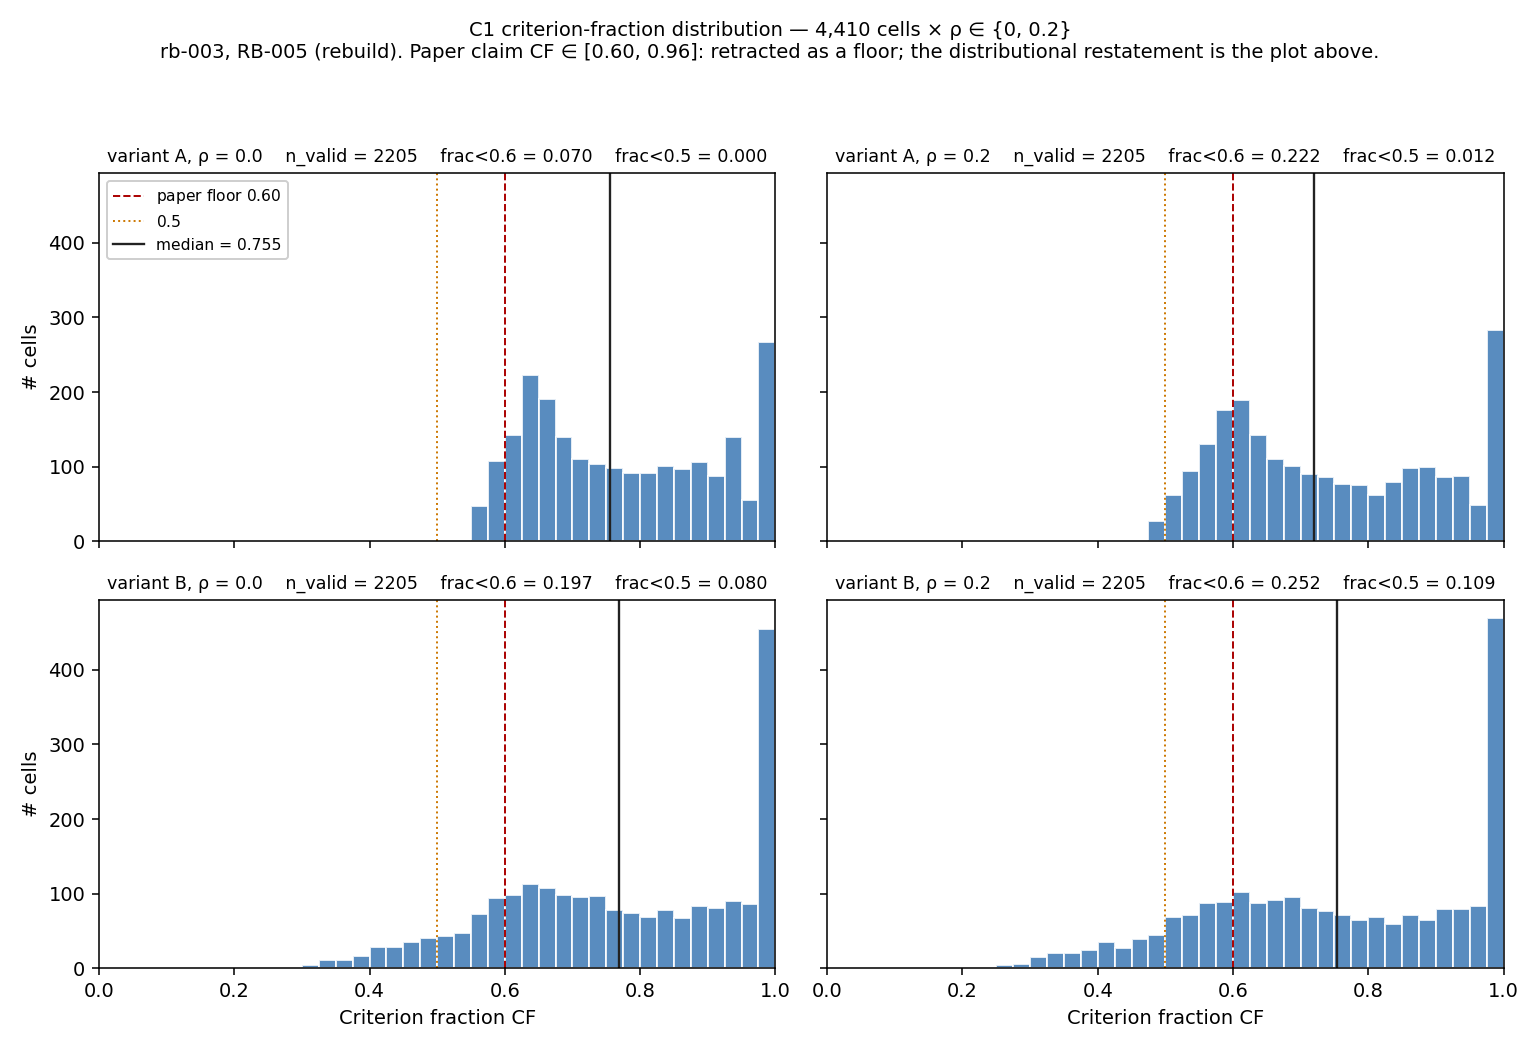
\includegraphics[width=0.95\linewidth]{figures/cf_histogram.png}
  \caption{Per-cell histogram of the criterion fraction $\CF$
  across the $4{,}410$-cell sweep (columns: variant; rows:
  $\corr \in \{0, 0.2\}$). Vertical dashed lines mark the inherited
  paper's stated floor $\CF = 0.60$ and ceiling $\CF = 0.96$
  (\texttt{Critique/source/main.pdf}, §5). The
  distributional shape --- a broad mode near $\CF \approx 0.65$, a
  left tail (much heavier in variant~B), and a spike at $\CF = 1$
  --- is the figure that replaces the inherited paper's categorical
  floor language. The $\corr = 0.2$ row exhibits the A1
  amplification of the left tail discussed below
  (Table~\ref{tab:cf-rho-sensitivity}). Reproduced from
  \texttt{Rebuild/sims/C1--cf-distribution/output/figures/cf\_histogram.png}.}
  \label{fig:cf-histogram}
\end{figure}

\paragraph{Where CF is high, where CF is low: a quadrant breakdown.}
The distributional summary of Table~\ref{tab:cf-distribution}
collapses across $(\Rsens, \valid)$ in a way that obscures the
\emph{regime} structure of $\CF$. To expose where the criterion
lever dominates and where it cedes to attention re-allocation, we
partition the cells into a $3 \times 2$ grid: $\Rsens$-regime
$\{\text{cost-dominant}\,(\Rsens < 1),\, \text{symmetric}\,
(\Rsens = 1),\, \text{benefit-dominant}\,(\Rsens > 1)\}$ crossed
with $\valid$-regime $\{\text{low validity}\,(\valid < 1/2),\,
\text{high validity}\,(\valid \ge 1/2)\}$. Table~\ref{tab:cf-quadrants}
reports the median $\CF$ within each quadrant at $\corr = 0$.
%
\begin{table}[t]
  \centering
  \small
  \begin{tabular}{l l r r r r}
    \toprule
    variant & $\Rsens$-regime &
    median $\CF$ & strict min &
    $\mathrm{frac}\!<\!0.6$ & $n$\\
    \midrule
    A & cost-dom., $\valid$ low   & $0.998$ & $0.825$ & $0.000$ & $350$\\
    A & cost-dom., $\valid$ high  & $0.897$ & $0.825$ & $0.000$ & $385$\\
    A & symmetric, $\valid$ low   & $0.779$ & $0.665$ & $0.000$ & $350$\\
    A & symmetric, $\valid$ high  & $0.740$ & $0.665$ & $0.000$ & $385$\\
    A & benefit-dom., $\valid$ high & $0.645$ & $0.563$ & $0.062$ & $385$\\
    A & benefit-dom., $\valid$ low  & $\mathbf{0.612}$ & $\mathbf{0.559}$
                                    & $\mathbf{0.374}$ & $350$\\
    \midrule
    B & cost-dom., $\valid$ low   & $1.000$ & $0.905$ & $0.000$ & $350$\\
    B & cost-dom., $\valid$ high  & $0.931$ & $0.797$ & $0.000$ & $385$\\
    B & symmetric, $\valid$ low   & $0.800$ & $0.497$ & $0.103$ & $350$\\
    B & symmetric, $\valid$ high  & $0.753$ & $0.575$ & $0.010$ & $385$\\
    B & benefit-dom., $\valid$ high & $0.630$ & $0.469$ & $0.317$ & $385$\\
    B & benefit-dom., $\valid$ low  & $\mathbf{0.509}$ & $\mathbf{0.304}$
                                    & $\mathbf{0.780}$ & $350$\\
    \bottomrule
  \end{tabular}
  \caption{Quadrant breakdown of $\CF$ at $\corr = 0$. The
  criterion lever dominates uniformly in the cost-dominant
  $\Rsens < 1$ region (median $\CF \ge 0.90$ in both variants) and
  cedes to attention re-allocation in the benefit-dominant,
  low-validity corner (variant~A: median $0.61$, 37\% of cells
  below $0.6$; variant~B: median $0.51$, 78\% of cells below
  $0.6$). The symmetric $\Rsens = 1$ row is intermediate and stable
  across variants. Block-keys
  \texttt{quadrant\_breakdown.rho\_0.0.<variant>/r=<r\_regime>/V=<V\_regime>}
  in \texttt{results.json}.}
  \label{tab:cf-quadrants}
\end{table}
%
The structure is consistent across variants: $\CF$ is monotonically
ordered ${\rm cost\text{-}dom.} > {\rm symmetric} > {\rm
benefit\text{-}dom.}$ along the $\Rsens$ axis, and within each
$\Rsens$-regime $\CF$ is reduced by lowering $\valid$. The
benefit-dominant low-validity corner is where the inherited paper's
categorical floor breaks: in variant~B this corner sits at median
$\CF = 0.51$ with $78\%$ of cells below $0.6$ and a strict minimum
of $0.30$. The same regime structure is visible cell-wise in
Figure~\ref{fig:cf-heatmap}, which displays the $(r, V)$-plane at
$\val = 5$ for each variant and each $\corr$, and in
Figure~\ref{fig:cf-curves}, which displays $\CF(\Rsens)$ at
$\valid \approx 0.5$ as a $\val$-family. The inherited paper's
qualitative ``CF $\to 1$ at small $r$, CF declines at large $r$''
intuition (\texttt{Critique/source/main.pdf}, §5) survives as the
generic $\Rsens$-axis ordering; what fails is the categorical
$[0.60, 0.96]$ bound on the resulting distribution.

\begin{figure}[t]
  \centering
  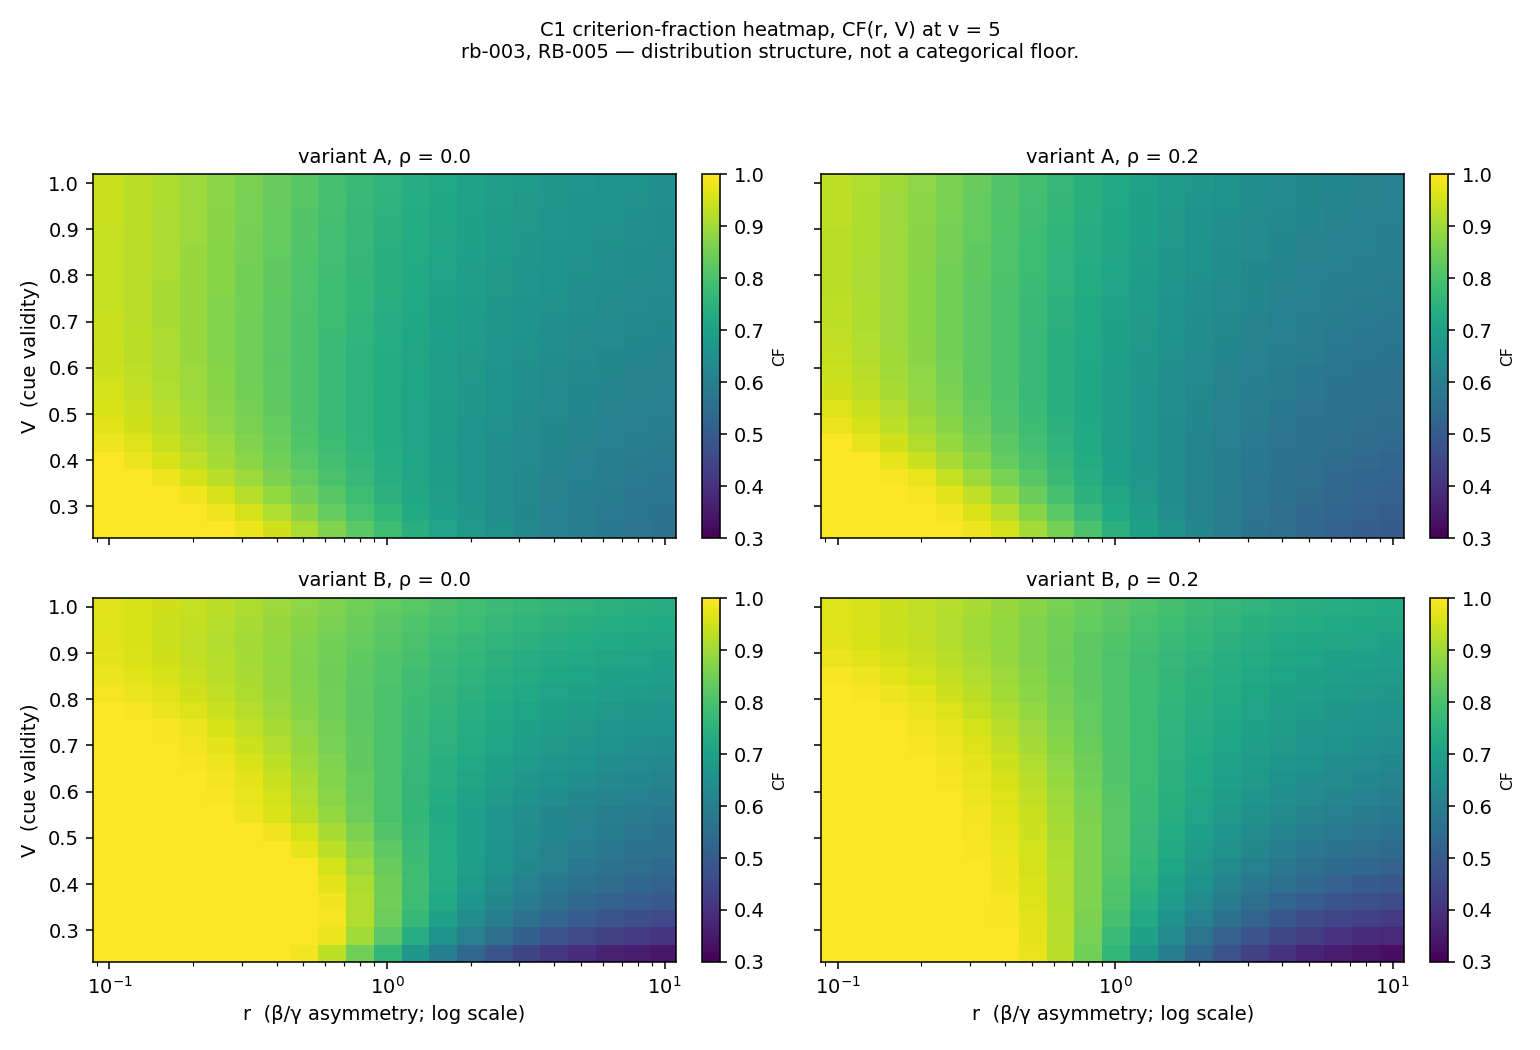
\includegraphics[width=0.95\linewidth]{figures/cf_heatmap.png}
  \caption{$\CF$ over the $(\Rsens, \valid)$-plane at $\val = 5$,
  $\Nloc = 4$, $\dprimemax = 2$, $f_0 = 0.5$, $h = \sqrt{\;\cdot\;}$
  (rows: $\corr$; columns: variant). The diagonal boundary in
  $(\log \Rsens,\,\valid)$ between the CF-near-$1$ low-$\Rsens$
  region (criterion-dominated) and the CF-low high-$\Rsens$
  low-$\valid$ corner (attention-dominated) is the regime
  structure quantified in Table~\ref{tab:cf-quadrants}. The
  low-CF corner is wider in variant~B and widens further at
  $\corr = 0.2$. Reproduced from
  \texttt{Rebuild/sims/C1--cf-distribution/output/figures/cf\_heatmap.png}.}
  \label{fig:cf-heatmap}
\end{figure}

\begin{figure}[t]
  \centering
  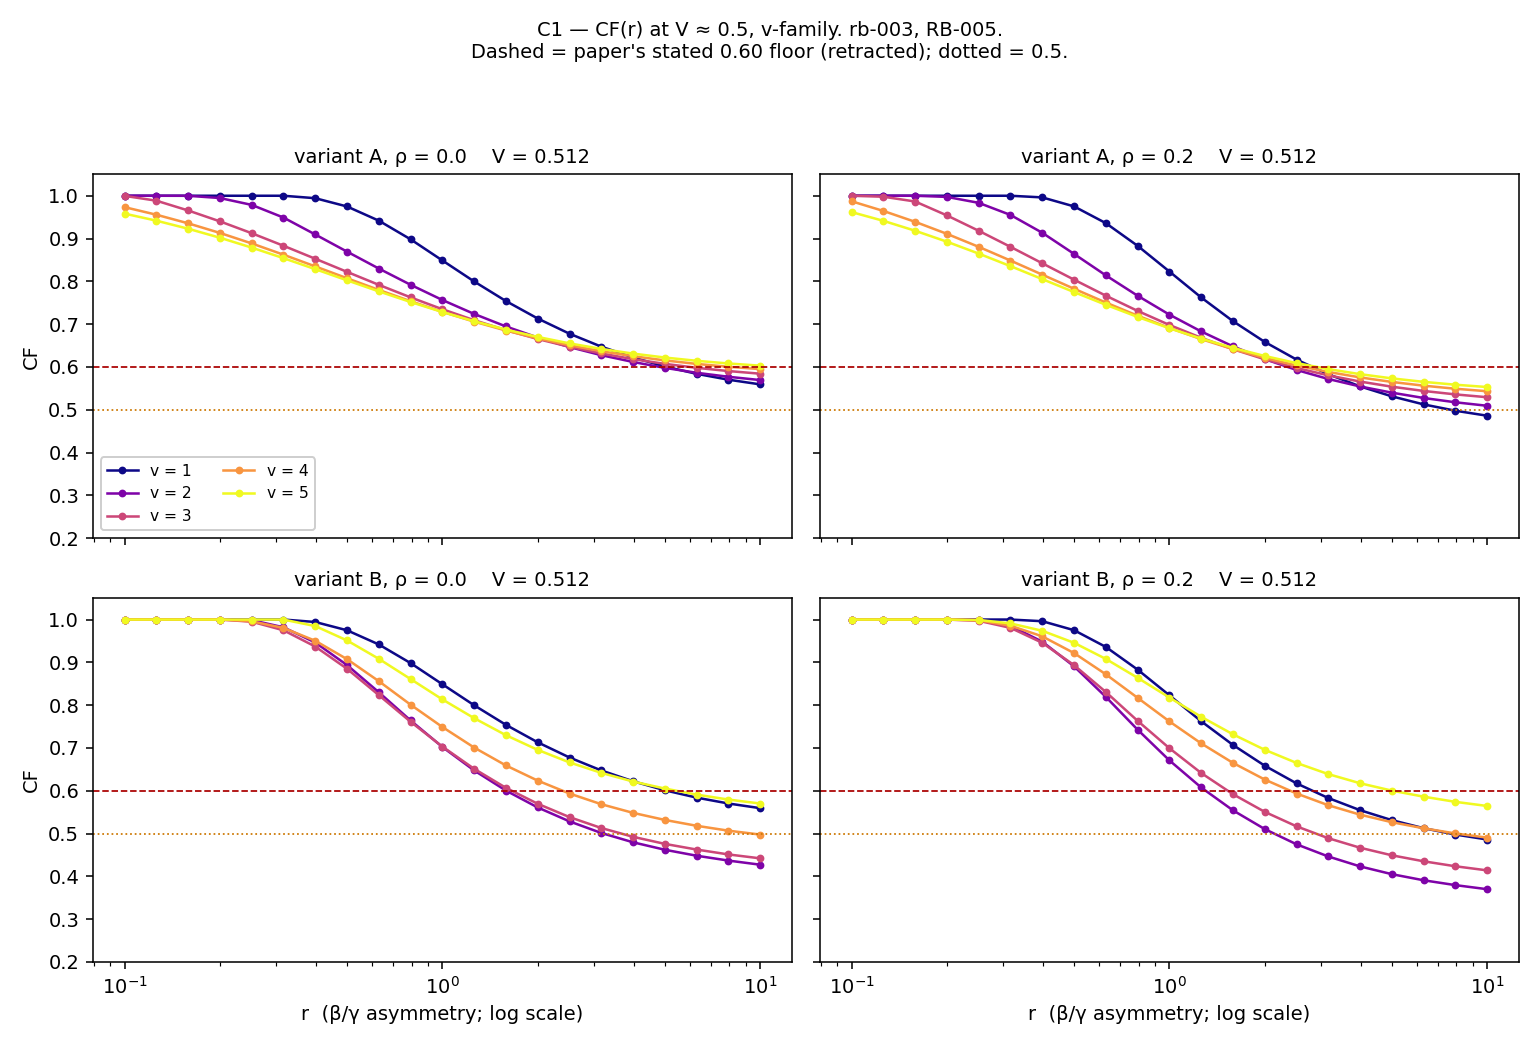
\includegraphics[width=0.95\linewidth]{figures/cf_curves.png}
  \caption{$\CF(\Rsens)$ at $\valid \approx 0.5$ as a $\val$-family
  $\val \in \{1, 2, 3, 4, 5\}$ (rows: $\corr$; columns: variant).
  At small $\Rsens$ (cost-dominant) the curves cluster near
  $\CF = 1$; as $\Rsens$ increases all curves decline, more steeply
  for larger $\val$, exposing the benefit-dominant region in which
  attention re-allocation overtakes the criterion shift. Reproduced
  from
  \texttt{Rebuild/sims/C1--cf-distribution/output/figures/cf\_curves.png}.}
  \label{fig:cf-curves}
\end{figure}

\paragraph{A1 sensitivity: $\corr$ amplifies the left tail in
variant~A; variant~B is mixed.}
The same $4{,}410$-cell sweep was repeated at $\corr = 0.2$ using
the rebuilt model's equicorrelated-Gaussian one-factor
Gauss--Hermite implementation (Section~\ref{sec:model}).
Per-variant marginals (Table~\ref{tab:cf-rho-sensitivity}) and a
cell-wise pairing (Table~\ref{tab:cf-delta-distribution}) are
reported.
%
\begin{table}[t]
  \centering
  \small
  \begin{tabular}{l c c c c c c c}
    \toprule
    variant & $\corr$ & $\CF_{\min}$ & median &
    $\mathrm{frac}\!<\!0.5$ & $\mathrm{frac}\!<\!0.6$ &
    $\mathrm{frac}\!<\!0.8$ & $\mathrm{frac}\!>\!0.9$\\
    \midrule
    A & $0.0$ & $0.5587$ & $0.7552$
      & $0.0000$ & $0.0703$ & $0.5701$ & $0.2499$\\
    A & $0.2$ & $0.4854$ & $0.7197$
      & $0.0122$ & $\mathbf{0.2222}$ & $0.6177$ & $0.2290$\\
    \midrule
    B & $0.0$ & $0.3040$ & $0.7682$
      & $0.0803$ & $0.1973$ & $0.5429$ & $0.3224$\\
    B & $0.2$ & $0.2406$ & $0.7538$
      & $0.1088$ & $0.2522$ & $0.5565$ & $0.3234$\\
    \bottomrule
  \end{tabular}
  \caption{Marginal CF distribution at $\corr \in \{0, 0.2\}$,
  per variant. The variant-A left tail amplifies by a factor of
  $\approx 3$ when $\corr$ is raised from $0$ to $0.2$
  ($\mathrm{frac}\!<\!0.6$: $0.07 \to 0.22$), and the variant-A
  strict minimum crosses below $0.5$ (it does not at $\corr = 0$).
  The variant-B marginals shift less dramatically: median moves by
  $-0.014$, $\mathrm{frac}\!<\!0.6$ by $+0.055$. Block-keys
  \texttt{summaries.variant\_<X>/rho\_<rho>}.}
  \label{tab:cf-rho-sensitivity}
\end{table}
%
\begin{table}[t]
  \centering
  \small
  \begin{tabular}{l c c c c c c}
    \toprule
    variant & frac dec. & frac inc. & frac flat &
    median $\Delta \CF$ & $|\Delta \CF|_{q_{95\%}}$ & $\Delta_{\min}$\\
    \midrule
    A & $\mathbf{0.8376}$ & $0.0834$ & $0.0789$ &
        $\mathbf{-0.0348}$ & $0.0640$ & $-0.0856$\\
    B & $0.6372$ & $\mathbf{0.2354}$ & $0.1274$ &
        $-0.0093$ & $0.0650$ & $-0.1068$\\
    \bottomrule
  \end{tabular}
  \caption{Cell-wise paired comparison
  $\Delta \CF := \CF(\corr{=}0.2) - \CF(\corr{=}0)$ across the
  $4{,}410$-cell sweep, per variant. ``Flat'' uses tolerance
  $|\Delta \CF| \le 10^{-5}$. The variant-A pattern is a one-sided
  ordering ($84\%$ of cells decrease in $\corr$). The variant-B
  pattern is mixed-sign ($64\%$ decrease, $24\%$ increase, $13\%$
  flat), generalising the rb-002 headline-cell observation that
  variant-B $\CF$ is essentially flat in $\corr$. Block-keys
  \texttt{delta\_distribution.<variant>}.}
  \label{tab:cf-delta-distribution}
\end{table}
%
The rebuilt model thus replaces the inherited paper's §5.5 claim
that independence \emph{upper-bounds VDA} (refuted at the headline
cell by rb-002 and the model section's $\corr$-sweep) with a
different and \emph{honestly variant-dependent} statement: at
variant~A, the independence assumption upper-bounds the
\emph{criterion fraction} $\CF$ on a strong majority of the primary
sweep ($84\%$ of cells; cell-wise median $\Delta \CF = -0.035$ when
$\corr$ is raised to $0.2$), but the bound is one-sided rather than
uniform ($8\%$ of cells move in the opposite direction). At
variant~B, the ordering fails as a general statement: only $64\%$
of cells decrease and $24\%$ increase, so independence
\emph{cannot} be claimed as a uniform upper bound on $\CF$ in
variant~B. This pattern is the cell-wise generalisation of the
rb-002 caveat that the variant-B headline-cell $\CF(\corr)$ is
essentially flat. We therefore state, here and in
Section~\ref{sec:model}, that the A1 channel reduces $\CF$ on a
typical variant-A cell and leaves $\CF$ essentially unchanged
(with substantial cell-wise scatter) on a typical variant-B cell;
the original §5.5 framing is retracted along this axis as well.

\paragraph{Scope and what is not yet claimed.}
The results in this subsection are reported at a single
$(\Nloc, \dprimemax, f_0, h) = (4, 2, 0.5, \sqrt{}\,)$
configuration and at the $\corr \in \{0, 0.2\}$ pair only. (i)~The
\emph{conservation-family band} on the headline CF numbers, in
which the additive ($\benefit + \cost = 2$) and multiplicative
($\benefit \cdot \cost = 1$) conservation rules are special cases
of a one-parameter family, is queued as RB-019 in
\texttt{REBUILD\_BACKLOG.md} and will be reported in
Section~\ref{sec:limitations} as a band on every number in
Tables~\ref{tab:cf-distribution}, \ref{tab:cf-quadrants}, and
\ref{tab:cf-rho-sensitivity}; the present subsection makes no
explicit conservation-family claim. (ii)~A finer $\corr$ grid (to
quantify the curvature of the variant-A $\CF$-versus-$\corr$
response and to sharpen the variant-B mixed-sign caveat) is queued
as RB-023. (iii)~A \emph{closed-form regime boundary} for the
CF-below-$0.5$ corner --- the heatmap of
Figure~\ref{fig:cf-heatmap} suggests a clean diagonal boundary in
$(\log \Rsens, \valid)$ in variant~B --- is queued as a derivation
increment RB-024; if it lands, the empirical statement
``$\mathrm{frac}\!<\!0.6 = 0.22$ at $\corr = 0.2$ in variant~A''
would be replaced by a closed-form predicate. (iv)~The cell-wise
$\val$-resolved sign-flip of $\partial \VDA / \partial \corr$
(rb-006, Table~\ref{tab:rho-sensitivity}) does not surface in this
subsection because $\CF$, not $\VDA$, is the headline quantity here;
the cell-wise VDA $\Delta$-distribution analogue is queued as RB-025.

\paragraph{Reproducibility.}
All numbers in Tables~\ref{tab:cf-distribution},
\ref{tab:cf-quadrants}, \ref{tab:cf-rho-sensitivity}, and
\ref{tab:cf-delta-distribution}, and all three figures, are
reproduced byte-for-byte by re-running
\texttt{Rebuild/sims/C1--cf-distribution/run.py}. The output digest
is \texttt{91fc4692dbc106eca9c90770c79e22f7f4757d76421ed55e7e8e91f80e44706c}
(\texttt{sha256} of the canonical-key-ordered numeric JSON,
excluding the digest field itself). The $\Phinorm$ backend is
\texttt{scipy.special.ndtr}; the criterion grid step is
$\Delta c = 0.05$ ($121$ points on $[-3, 3]$); the $\alpha$ grid
step is $\Delta \alpha = 0.02$ ($51$ points on $[0, 1]$, matching
the reviewer's CR-002 substrate); the $(\Rsens, \valid, \val)$
grid is the $21 \times 21 \times 5$ grid described above; both
variants ($\benefit + \cost = 2$; $\benefit \cdot \cost = 1$) and
both correlations ($\corr \in \{0, 0.2\}$) are evaluated; runtime
$\approx 67$~s on the rebuild's reference machine. The recovery
test against the reviewer's
\texttt{Critique/replications/C1--criterion-fraction-floor/output/results.json}
passes cell-wise at $\max|\Delta \CF| = 1.47 \times 10^{-6}$ and
$\max|\Delta \Rew_{\mathrm{P1..P4}}| \le 5.65 \times 10^{-7}$
across all $4{,}410$ cells; the gap is a known ULP-scale
\texttt{1 - Phi(-b)} versus \texttt{Phi(b)} reordering in the
reviewer's \texttt{floor\_R}, well past the four-decimal precision
of any reported number.

% ---------------------------------------------------------------------
\subsection{Non-monotonicity of VDA in $\Rsens$ with closed-form
            escape threshold (C2)}
\label{sec:results-c2}

\paragraph{Claim restated at defensible strength.}
The inherited paper presents the non-monotonicity of the
value-directed attention benefit
$\VDA(\Rsens) := \Rpone(\Rsens) - \Rptwo(\Rsens)$
in the benefit/cost ratio $\Rsens$ as the central finding of its
results: $\VDA$ rises out of zero at small $\Rsens$, peaks in an
interior region, then decays back to zero as $\Rsens \to \infty$.
The live skeptical-reviewer verdict for this claim
(\texttt{Critique/verdicts/C2--non-monotonic-vda.md},
\texttt{current\_label: CONFIRMED-UNDER-ATTACK}) records that the
claim survives both re-derivation and a sensitivity attack along
$\val$ and $f_0$. We therefore retain the claim at full strength in
the rebuild, and \emph{strengthen} it by promoting the underlying
mechanism --- which the inherited paper described qualitatively ---
into a closed-form display.

\paragraph{Closed-form escape threshold.}
Differentiating the expected reward $\Rpone(\alpha, \Rsens)$ at the
uniform allocation $\alpha = 1/\Nloc$, the first-order condition for
P1 to leave the uniform interior $\partial_\alpha \Rpone|_{1/\Nloc} =
0$ defines a critical value of the benefit/cost ratio at which the
optimiser begins to re-allocate attention toward the cued location.
Writing $\dprime_b := \dprimemax\, f(1/\Nloc)$ for the baseline
discriminability at uniform attention and $(c_c^\star, c_u^\star)$
for the per-policy P3-optimal criterion pair at $\alpha = 1/\Nloc$,
the threshold takes the form
%
\begin{equation}
  \rdagger(\val) \;=\; \frac{K_u(\val)}{(\Nloc - 1) \cdot K_c(\val)},
  \label{eq:r-dagger}
\end{equation}
%
where the per-location gradient coefficients are
%
\begin{align}
  K_c(\val) &= \tfrac{1}{4}\Big[
    \valid\, \val\, \phi\!\big(\tfrac{\dprime_b}{2} - c_c^\star\big)
    \;+\; \CR(\val)\, \phi\!\big(\tfrac{\dprime_b}{2} + c_c^\star\big)\,
    \Phinorm\!\big(\tfrac{\dprime_b}{2} + c_u^\star\big)^{\Nloc - 1}
  \Big],
  \label{eq:K-c}
  \\[2pt]
  K_u(\val) &= \tfrac{1}{4}\Big[
    (1 - \valid)\, \phi\!\big(\tfrac{\dprime_b}{2} - c_u^\star\big)
    \;+\; (\Nloc - 1)\, \CR(\val)\, \Phinorm\!\big(\tfrac{\dprime_b}{2}
    + c_c^\star\big)
    \notag\\
    &\qquad\quad\;\;\;\;\;\;\;\;\;\;\;\;\;\;\;\;\;\;\;\;\;\;\;
    \cdot\, \Phinorm\!\big(\tfrac{\dprime_b}{2} + c_u^\star\big)^{\Nloc - 2}
    \phi\!\big(\tfrac{\dprime_b}{2} + c_u^\star\big)
  \Big].
  \label{eq:K-u}
\end{align}
%
The conservation indicator $\CR(\val)$ encodes the
benefit-vs-correct-rejection scaling (under variant A,
$\benefit(\Rsens) + \cost(\Rsens) = 2$, the value-blind correct
rejection scales as $\CR(\val) = 1$; the variant-B multiplicative
conservation $\benefit\,\cost = 1$ is treated as a sensitivity in
Section~\ref{sec:limitations}). The independent re-derivation of
\eqref{eq:r-dagger}--\eqref{eq:K-u} from
$\partial_\alpha \Rpone(\alpha, \Rsens) |_{\alpha = 1/\Nloc} = 0$ is
deferred to Section~\ref{sec:appendix-deriv-c2}. The threshold is a
theorem of the model definitions, not an empirical regularity.

\paragraph{Numerical $\val$-family at the headline cell.}
At the C2 headline cell
$(\Nloc, \dprimemax, f_0, h, \valid) = (4,\,2,\,0.5,\,\sqrt{},\,0.5)$
under variant~A, equations \eqref{eq:r-dagger}--\eqref{eq:K-u}
evaluate to the values in Table~\ref{tab:r-dagger-family}.
%
\begin{table}[t]
  \centering
  \small
  \begin{tabular}{r r r r r r}
    \toprule
    $\val$ &
    $\rdagger(\val)$ &
    $c_c^\star$ &
    $c_u^\star$ &
    $K_c(\val)$ &
    $K_u(\val)$ \\
    \midrule
    $1$  & $0.343$ & $\phantom{-}0.40$ & $1.05$ & $0.0930$ & $0.0958$ \\
    $2$  & $0.168$ & $\phantom{-}0.25$ & $1.30$ & $0.1734$ & $0.0872$ \\
    $3$  & $0.099$ & $\phantom{-}0.15$ & $1.50$ & $0.2532$ & $0.0755$ \\
    $5$  & $0.050$ & $\phantom{-}0.10$ & $1.75$ & $0.4065$ & $0.0615$ \\
    $8$  & $0.022$ & $\phantom{-}0.05$ & $2.05$ & $0.6357$ & $0.0424$ \\
    $10$ & $0.016$ & $\phantom{-}0.05$ & $2.15$ & $0.7864$ & $0.0380$ \\
    \bottomrule
  \end{tabular}
  \caption{Closed-form escape threshold $\rdagger(\val) = K_u(\val) /
  [(\Nloc - 1)\,K_c(\val)]$ from \eqref{eq:r-dagger}--\eqref{eq:K-u}
  at the C2 headline cell. The $\val = 1$ row is the symmetric
  reference $\rdagger(1) \approx 0.343$. Values from
  \texttt{Rebuild/sims/C2--vda-vs-r-vfamily/output/results.json}
  (rb-004; output sha256 \texttt{09ecef3c\ldots}).}
  \label{tab:r-dagger-family}
\end{table}
%
The threshold is monotone-decreasing in the cued value $\val$,
spanning roughly $\rdagger(2) \approx 0.17$ down to $\rdagger(10)
\approx 0.02$. Figure~\ref{fig:r-dagger-vs-v} plots
$\rdagger(\val)$ on a continuous $\val$-trace with the family points
of Table~\ref{tab:r-dagger-family} highlighted.
%
\begin{figure}[t]
  \centering
  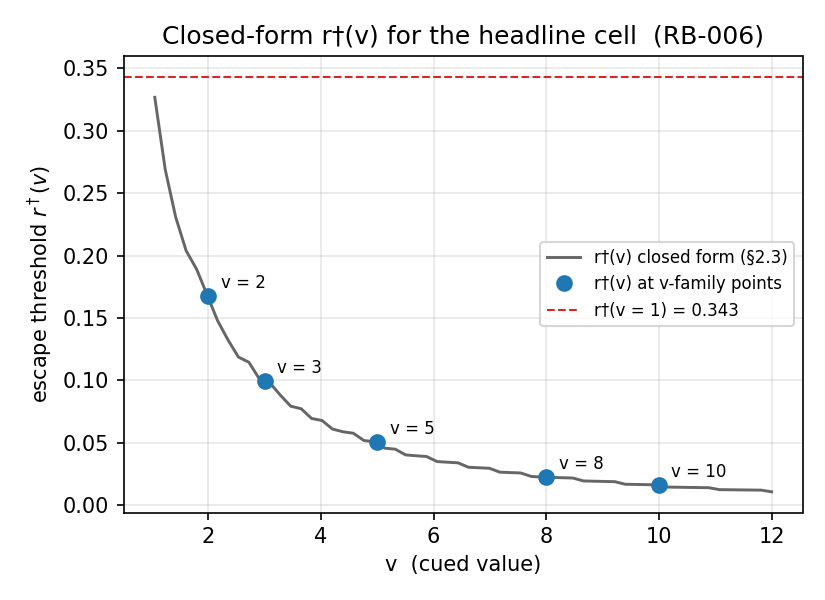
\includegraphics[width=0.7\linewidth]{figures/r_dagger_vs_v.png}
  \caption{Closed-form VDA-escape threshold $\rdagger(\val)$ at the
  headline cell $(\Nloc, \dprimemax, f_0, h, \valid) =
  (4,\,2,\,0.5,\,\sqrt{},\,0.5)$, variant~A. Continuous trace
  computed from \eqref{eq:r-dagger}--\eqref{eq:K-u} on a dense
  $\val$-grid; family points $\val \in \{2,3,5,8,10\}$
  marked. The horizontal reference $\rdagger(1) \approx 0.343$
  is the symmetric upper anchor of the family.
  Reproduced from
  \texttt{Rebuild/sims/C2--vda-vs-r-vfamily/output/figures/r\_dagger\_vs\_v.png}.}
  \label{fig:r-dagger-vs-v}
\end{figure}

\paragraph{Empirical confirmation: the peak lies above
$\rdagger(\val)$.}
The closed-form threshold marks the $\Rsens$ value at which P1
\emph{begins} to depart from uniform attention. The peak of $\VDA$,
by contrast, occurs at the (larger) $\Rsens$ at which P1's
re-allocation gain has built up most strongly against the still-locked
value-blind baseline P2 --- which in turn departs uniform attention at
the higher threshold $\rdagger(\val = 1)$ (the symmetric case in
Table~\ref{tab:r-dagger-family}). The non-monotonicity arises because
$\VDA$ opens up in the interior interval $(\rdagger(\val),\,
\rdagger(1))$ and decays once P2 also escapes uniform attention. A
high-resolution sweep
($\Rsens$-grid of $84$ log-spaced points, including the rb-002 pins
$\{0.398, 1.000, 3.162\}$ and the new finer-grid peak pin
$\Rsens = 0.3831$) confirms the prediction
$r^\star > \rdagger(\val)$ for every $\val$ in the family
(Table~\ref{tab:peak-vs-threshold}).
%
\begin{table}[t]
  \centering
  \small
  \begin{tabular}{r r r r c}
    \toprule
    $\val$ &
    $\rdagger(\val)$ &
    $r^\star$ &
    $r^\star - \rdagger(\val)$ &
    above? \\
    \midrule
    $2$  & $0.168$ & $0.501$ & $+0.334$ & \checkmark \\
    $3$  & $0.099$ & $0.376$ & $+0.276$ & \checkmark \\
    $5$  & $0.050$ & $0.376$ & $+0.325$ & \checkmark \\
    $8$  & $0.022$ & $0.376$ & $+0.354$ & \checkmark \\
    $10$ & $0.016$ & $0.355$ & $+0.339$ & \checkmark \\
    \bottomrule
  \end{tabular}
  \caption{Empirical peak $r^\star = \arg\max_{\Rsens} \VDA(\Rsens)$
  vs.\ closed-form escape threshold $\rdagger(\val)$ at the headline
  cell, $\corr = 0$. The peak $r^\star$ lies above $\rdagger(\val)$
  for every $\val$ and clusters near
  $\rdagger(\val{=}1) \approx 0.343$, consistent with the prediction
  that $\VDA$ is supported on the interior interval
  $(\rdagger(\val),\,\rdagger(1))$. Numerical resolution: peak
  $r^\star$ on an $84$-point log-grid; recovery against the rb-002
  reference at $r \in \{0.398, 1.000, 3.162\}$ at
  $\max|\Delta\VDA| = 4.87 \times 10^{-6}$.}
  \label{tab:peak-vs-threshold}
\end{table}

Figure~\ref{fig:vda-curves-vfamily} reproduces the full $\VDA(\Rsens)$
family. The left panel ($\corr = 0$) shows the inherited model: an
interior peak that grows monotonically with $\val$, from peak
$\VDA \approx 0.012$ at $\val = 2$ to peak
$\VDA \approx 0.183$ at $\val = 10$, with each peak sitting above
the corresponding $\rdagger(\val)$ vertical (dashed). The right panel
plots the same family at $\corr = 0.2$, foreshadowing the A1
sensitivity paragraph below.

\begin{figure}[t]
  \centering
  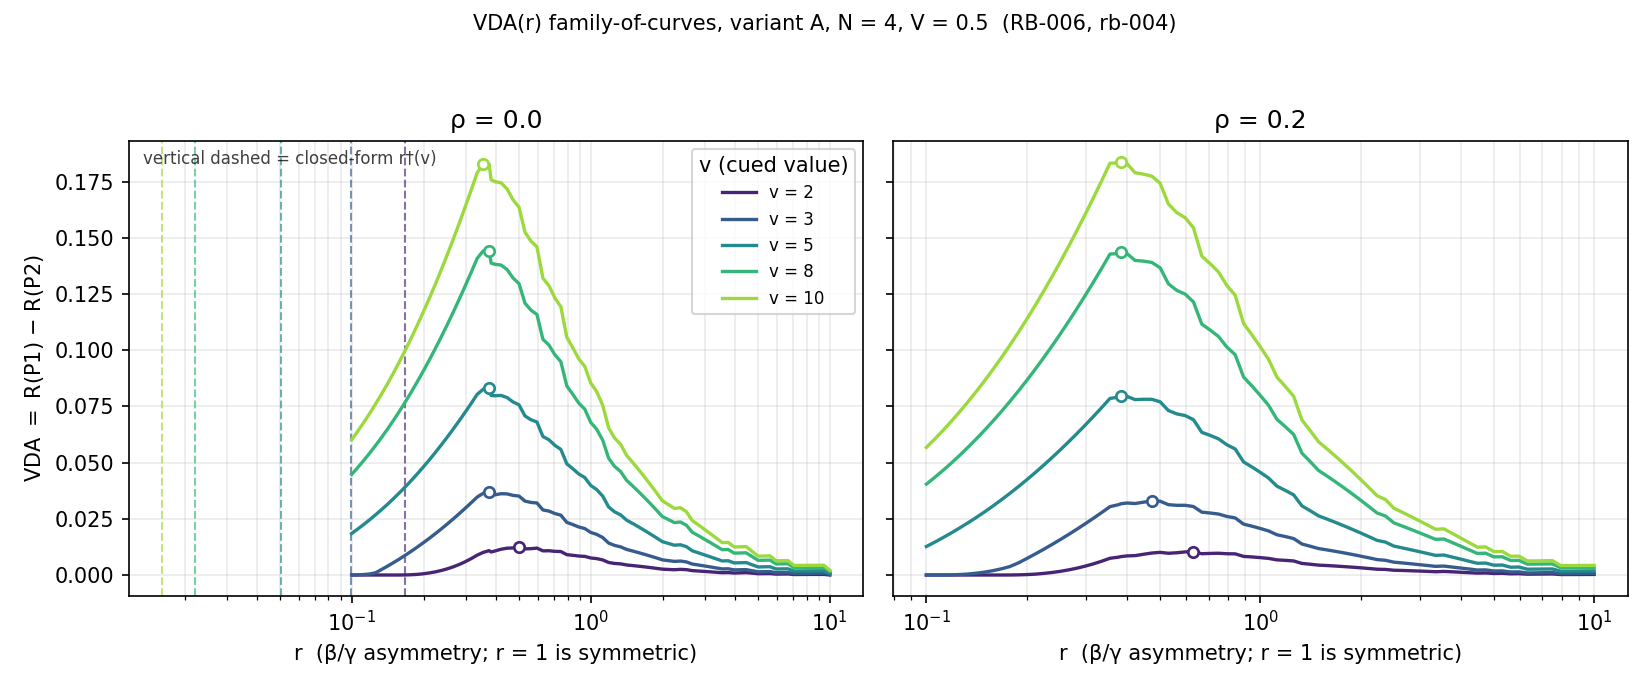
\includegraphics[width=0.95\linewidth]{figures/vda_curves_vfamily.png}
  \caption{Non-monotonicity of $\VDA(\Rsens)$ in the benefit/cost
  ratio across a $\val$-family at the headline cell
  $(\Nloc, \dprimemax, f_0, h, \valid) = (4, 2, 0.5, \sqrt{}, 0.5)$,
  variant~A. Left: $\corr = 0$ (the inherited independent model);
  the closed-form escape threshold $\rdagger(\val)$ from
  \eqref{eq:r-dagger} is overlaid as a vertical dashed line for each
  $\val$, and the empirical peak (white-filled dot) lies above
  $\rdagger(\val)$ for every $\val$ in the family (cf.\
  Table~\ref{tab:peak-vs-threshold}). Right: same family at
  $\corr = 0.2$ --- the A1 decorrelation channel suppresses the peak
  at low $\val$ but amplifies it at $\val = 10$ (cf.\
  Table~\ref{tab:rho-sensitivity}); the sign of
  $\partial \VDA^\star/\partial \corr$ depends on $\val$, not just
  on $\Rsens$.
  Reproduced from
  \texttt{Rebuild/sims/C2--vda-vs-r-vfamily/output/figures/vda\_curves\_vfamily.png}.}
  \label{fig:vda-curves-vfamily}
\end{figure}

\paragraph{A1 sensitivity: $\val$-dependent sign-flip of
$\partial \VDA^\star / \partial \corr$.}
The earlier sub-result rb-002, at a single headline cell, found that
introducing cross-location correlation $\corr$ shifts the sign of
$\partial \VDA / \partial \corr$ across $\Rsens$: $\corr$
\emph{suppresses} VDA in the cost-dominant regime
($\Rsens \lesssim 0.4$) but \emph{amplifies} it in the
benefit-dominant regime ($\Rsens \gtrsim 0.5$). The present
$\val$-family sweep generalises this finding from a sign-flip
along $\Rsens$ to a sign-flip along $\val$: at the empirical peak,
holding everything else fixed, the change in peak $\VDA$ when
$\corr$ is raised from $0$ to $0.2$ is reported in
Table~\ref{tab:rho-sensitivity}.
%
\begin{table}[t]
  \centering
  \small
  \begin{tabular}{r r r r r r}
    \toprule
    $\val$ &
    $\VDA^\star\,(\corr{=}0)$ &
    $\VDA^\star\,(\corr{=}0.2)$ &
    $\Delta \VDA^\star$ &
    $r^\star\,(\corr{=}0)$ &
    $r^\star\,(\corr{=}0.2)$ \\
    \midrule
    $2$  & $0.01233$ & $0.01036$ & $-0.00197$ & $0.501$ & $0.631$ \\
    $3$  & $0.03698$ & $0.03291$ & $-0.00407$ & $0.376$ & $0.473$ \\
    $5$  & $0.08300$ & $0.07954$ & $-0.00345$ & $0.376$ & $0.383$ \\
    $8$  & $0.14422$ & $0.14355$ & $-0.00067$ & $0.376$ & $0.383$ \\
    $10$ & $0.18284$ & $0.18387$ & $\mathbf{+0.00103}$ & $0.355$ & $0.383$ \\
    \bottomrule
  \end{tabular}
  \caption{A1 sensitivity at the empirical peak. $\corr = 0.2$
  suppresses peak $\VDA$ for $\val \le 8$ and amplifies at $\val = 10$.
  The peak location $r^\star$ also drifts upward in $\corr$, most
  visibly at low $\val$ ($r^\star$ rises from $0.501$ to $0.631$ at
  $\val = 2$). The $\val$-dependent sign-flip of
  $\partial \VDA^\star / \partial \corr$ is the $\val$-axis analogue
  of the $\Rsens$-axis sign-flip rb-002 reported at fixed $\val = 5$.
  Numerical recovery of the $\corr = 0$ row against rb-002 reference
  pins at $r \in \{0.398, 1.000, 3.162\}$ is at $\max|\Delta\VDA| =
  4.87 \times 10^{-6}$ (rb-004 recovery block).}
  \label{tab:rho-sensitivity}
\end{table}
%
The empirical $\corr$-drift of $r^\star$ in
Table~\ref{tab:rho-sensitivity} is the peak-location counterpart
of a closed-form drift of the \emph{escape-band lower edge}: the
$\corr > 0$ extension of \eqref{eq:r-dagger}--\eqref{eq:K-u}
derived in Section~\ref{sec:appendix-deriv-c2} (Proposition
\ref{prop:r-dagger-rho}, Equation~\eqref{eq:r-dagger-rho}) replaces
the no-FA terms inside $K_c, K_u$ with their $\corr$-aware 1-D
Gauss--Hermite gradients $I_c(b_c, b_u; \corr, \Nloc)$ and
$I_u(b_c, b_u; \corr, \Nloc)$ (Equations~\eqref{eq:c2-Ic}--\eqref{eq:c2-Iu})
and yields a closed form for $\rdagger(\val; \corr)$. Evaluated at
the headline cell, the closed form predicts $\rdagger(\val;0.2) >
\rdagger(\val;0)$ at every $\val \in \{1, 2, 3, 5, 8, 10\}$ (drift
fraction $+3\%$ at $\val = 1$ up to $+30\%$ at $\val = 8$;
Table~\ref{tab:r-dagger-rho-drift}). The sign of the closed-form
drift $\Delta\rdagger$ matches the sign of the empirical peak drift
$\Delta r^\star$ of Table~\ref{tab:rho-sensitivity} at all five rows
$\val \ne 1$; the lower edge cannot exceed the peak, so the
analytic upward drift of $\rdagger(\val;\corr)$ is the
mechanistic substrate of the empirical upward drift of
$r^\star(\val;\corr)$. A parallel cell-wise generalisation of the
sign-flip across the broader 4,410-cell sweep is queued as a
sensitivity increment (RB-025 in \texttt{REBUILD\_BACKLOG.md}).
What Table~\ref{tab:rho-sensitivity} and the closed form of
Section~\ref{sec:appendix-deriv-c2} jointly license is a
directional statement at the appropriate strength: under the A1
decorrelation lever, the C2 non-monotonicity \emph{is not}
uniformly attenuated; in the strongly benefit-dominant, high-value
corner the lever \emph{enhances} VDA, and the
escape-band lower edge drifts upward across the full $\val$-family.
The original paper's §5.5 framing of independence as an
\emph{upper bound on VDA} is therefore retracted along this axis,
consistent with the A1 row of \texttt{CLAIM\_LEDGER.md}.

\paragraph{Scope and what is not yet claimed.}
The results in this subsection are reported under variant~A
(additive conservation, $\benefit + \cost = 2$,
$\CR(\val) = 1$). The variant-B replication of the $\val$-family
sweep is queued as RB-027 in \texttt{REBUILD\_BACKLOG.md} and will
be reported in Section~\ref{sec:limitations} as part of the
conservation-family sensitivity band; the present subsection makes
no variant-B claim. The closed-form $\rdagger(\val; \corr > 0)$
derivation that mechanistically underwrites the upward drift of
$r^\star$ in $\corr$ in Table~\ref{tab:rho-sensitivity} is recorded
in Section~\ref{sec:appendix-deriv-c2}
(Proposition~\ref{prop:r-dagger-rho},
Table~\ref{tab:r-dagger-rho-drift}); the present subsection
reports the peak-location drift, not the lower-edge drift, as
data.
The conservation-family band on the peak $\VDA^\star$ magnitudes ---
once the A3 generalisation lands (RB-019) --- will replace the
single-conservation peak values reported in
Table~\ref{tab:peak-vs-threshold} with a band; we flag this here so
the reader knows the present headline magnitudes are conditional on
variant~A.

\paragraph{Reproducibility.}
All numbers in Tables~\ref{tab:r-dagger-family},
\ref{tab:peak-vs-threshold}, and \ref{tab:rho-sensitivity}, and both
figures, are reproduced byte-for-byte by re-running
\texttt{Rebuild/sims/C2--vda-vs-r-vfamily/run.py}. The output digest
is \texttt{09ecef3c2c5a101820951398ed7d6e67d3398aede80c5f0bddfa42b6224fd783}
(\texttt{sha256} of the canonical-key-ordered numeric JSON,
excluding the digest field itself). The Phi backend is
\texttt{scipy.special.ndtr}; the criterion grid step is
$\Delta c = 0.05$; the $\alpha$ grid step is
$\Delta\alpha = 0.005$; the $\Rsens$-grid is 84 log-spaced points
including the rb-002 pins and the new $\Rsens = 0.3831$ peak pin;
$\corr \in \{0, 0.2\}$. Recovery against rb-002 passes at every
pinned $r$ value at $|\Delta \VDA| \le 6 \times 10^{-6}$ and at
$|\Delta \CF| \le 2 \times 10^{-6}$; the finer-grid argmax raises
the rb-002 peak from $\VDA = 0.07986$ at $\Rsens = 0.3831$ to
$\VDA = 0.08300$ at $\Rsens = 0.3758$, a grid-density refinement
gain, not a regression.

% ---------------------------------------------------------------------
\subsection{Graded regime boundary (C3)}
\label{sec:results-c3}

\paragraph{Claim restated at defensible strength.}
The inherited paper characterises the regime in which VDA is large as
\emph{narrow}: VDA concentrates at low cue validity $\valid \approx
1/\Nloc$, high value contrast $\val \gg 1$, and moderate
benefit/cost asymmetry $\Rsens$. From that qualitative picture, §5.2
of the inherited manuscript
(\texttt{Critique/source/main.pdf}) draws a \textbf{categorical}
experimental-design implication: standard spatial cueing paradigms
with high validity ($\valid \ge 0.75$) are predicted to show
\emph{negligible VDA regardless of other parameters}. The live
skeptical-reviewer verdict for this claim
(\texttt{Critique/verdicts/C3--narrow-regime.md},
\texttt{current\_label: CONTESTED}) records that the qualitative
``narrow regime'' reading is sustained but the categorical §5.2
implication is too strong --- it holds only when ``high validity'' is
operationalised at a threshold strictly above the inherited $\valid
\ge 0.75$, and only under a $\corr$-conditional caveat. The rebuilt
C3 is therefore presented in this section as a \emph{graded /
quantitative} statement: a contour band over the experimental-design
plane $(\valid, \val)$ that quantifies exactly how the peak VDA
falls off as the design moves into the high-validity stratum, and an
explicit replacement for the §5.2 sentence that hedges the validity
threshold and the $\corr$-conditional caveat. The A1 decorrelation
channel $\corr$ is reported alongside the contour map as a
sensitivity --- the convention established in Section~\ref{sec:results}.

\paragraph{Iso-VDA contour band over $(\valid, \val)$.}
The rebuilt model was evaluated at the headline configuration
$(\Nloc, \dprimemax, f_0, h) = (4,\,2,\,0.5,\,\sqrt{}\,)$ under
variant~A on a grid of $\valid \in [0.25, 1.00]$ ($31$ uniform
points, step $0.025$), $\val \in [1.0, 10.0]$ ($19$ uniform points,
step $0.5$), $\Rsens \in \{0.3,\, 1,\, 3\}$ (three asymmetry strata:
cost-dominant moderate, symmetric, benefit-dominant), and $\corr \in
\{0,\, 0.2\}$ (independent baseline plus the
Cohen--Maunsell~\cite{CohenMaunsell2009} $r_{SC} \approx 0.2$ V4
anchor), for a total of $31 \times 19 \times 3 \times 2 = 3{,}534$
$(\valid, \val, \Rsens, \corr)$-cells. Per cell, the rebuilt
\texttt{policies()} call returns the optimal allocation, criteria,
and the four nested-policy expected rewards
$\Rew_{\mathrm{P1..P4}}$ from which $\VDA = \Rpone - \Rptwo$ is
formed. Figure~\ref{fig:iso-vda-contours} presents the resulting
iso-VDA contour band as a $2 \times 3$ panel grid (rows: $\corr$,
columns: $\Rsens$).
%
\begin{figure}[t]
  \centering
  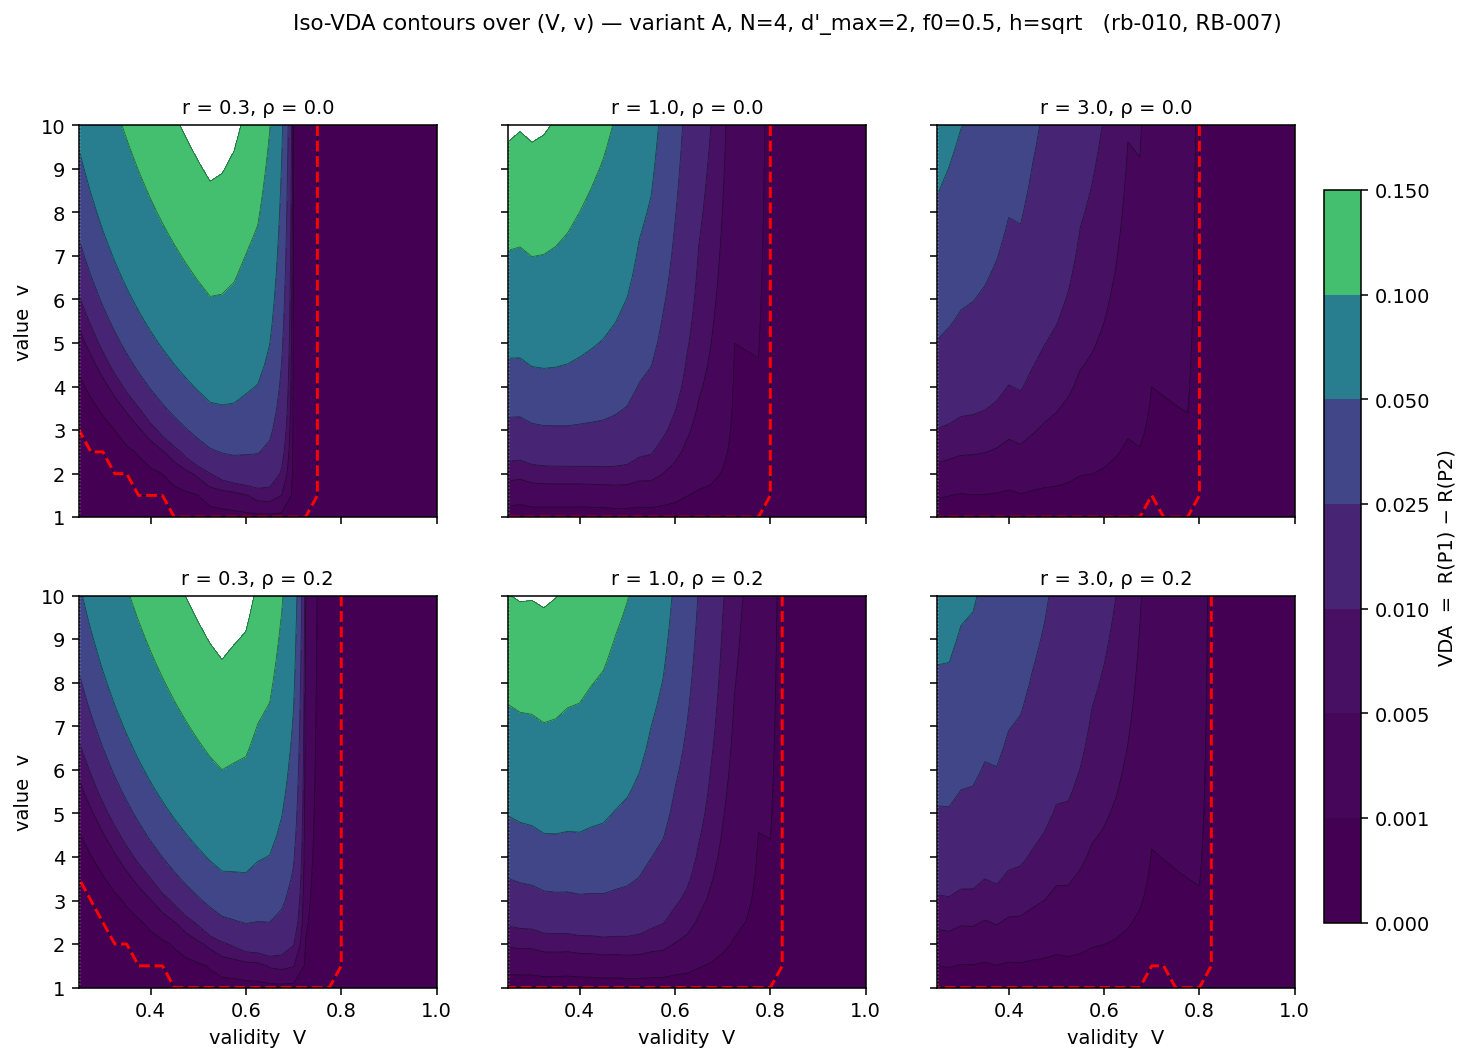
\includegraphics[width=0.98\linewidth]{figures/iso_vda_contours.png}
  \caption{Iso-VDA contour band over the experimental-design plane
  $(\valid, \val)$ for the rebuilt model at the headline cell
  $(\Nloc, \dprimemax, f_0, h) = (4,\,2,\,0.5,\,\sqrt{}\,)$,
  variant~A. Rows: cross-location correlation $\corr \in \{0,\,
  0.2\}$ (top: inherited independent model; bottom: with the A1
  decorrelation channel of Section~\ref{sec:model} at the
  Cohen--Maunsell~\cite{CohenMaunsell2009} V4 anchor $r_{SC}
  \approx 0.2$). Columns: benefit/cost asymmetry $\Rsens \in
  \{0.3,\, 1,\, 3\}$ (cost-dominant, symmetric, benefit-dominant).
  The vertical reference $\valid = 1/\Nloc = 0.25$ is the chance
  baseline; the $\val = 1$ row is the value-blind reference where
  $\VDA \equiv 0$ by construction. Filled contours are at $\VDA \in
  \{0,\,0.001,\,0.005,\,0.01,\,0.025,\,0.05,\,0.1,\,0.15,\,0.2\}$
  on a common scale. The band shape replaces the inherited §4
  ``narrow regime'' description and §5.2 categorical claim with a
  quantitative boundary the reader can compute pointwise. Reproduced
  from
  \texttt{Rebuild/sims/C3--iso-vda-Vv/output/figures/iso\_vda\_contours.png}
  (rb-010; output sha256 \texttt{72820559\ldots}).}
  \label{fig:iso-vda-contours}
\end{figure}
%
The qualitative ``narrow regime'' reading of the inherited paper is
visible directly: in every panel, the bulk of $(\valid, \val)$ space
carries near-zero VDA (median $\VDA \le 0.007$ in every panel; see
Table~\ref{tab:c3-marginals}), and substantial VDA is confined to a
\emph{corner} along low $\valid$ and high $\val$. The corner
\emph{flattens} along the $\Rsens$-axis: at the cost-dominant column
$\Rsens = 0.3$ the corner is broad and reaches $\VDA \approx 0.17$;
at the symmetric column $\Rsens = 1$ it narrows to $\VDA \approx
0.16$; at the benefit-dominant column $\Rsens = 3$ it collapses
sharply ($\VDA \le 0.06$ everywhere on the grid). The $\corr = 0.2$
row is read off below as the A1 sensitivity.

\paragraph{Distributional summary across panels.}
The per-panel distribution of $\VDA$ across the $589 = 31 \times 19$
$(\valid, \val)$-cells in each panel is summarised in
Table~\ref{tab:c3-marginals}.
%
\begin{table}[t]
  \centering
  \small
  \begin{tabular}{c c c c c c c c}
    \toprule
    $\Rsens$ & $\corr$ &
    $\VDA_{\min}$ & median & $q_{95\%}$ & $\VDA_{\max}$ &
    $\mathrm{frac}\!\ge\!0.005$ & $\mathrm{frac}\!\ge\!0.05$ \\
    \midrule
    $0.3$ & $0.0$ & $0$ & $0.0010$ & $0.1289$ & $\mathbf{0.1734}$ & $0.465$ & $0.287$\\
    $0.3$ & $0.2$ & $0$ & $0.0040$ & $0.1328$ & $\mathbf{0.1780}$ & $0.484$ & $0.295$\\
    \midrule
    $1.0$ & $0.0$ & $0$ & $0.0052$ & $0.1152$ & $0.1574$ & $0.503$ & $0.219$\\
    $1.0$ & $0.2$ & $0$ & $0.0069$ & $0.1180$ & $0.1552$ & $0.535$ & $0.236$\\
    \midrule
    $3.0$ & $0.0$ & $0$ & $0.0024$ & $0.0361$ & $0.0619$ & $0.380$ & $0.012$\\
    $3.0$ & $0.2$ & $0$ & $0.0025$ & $0.0390$ & $0.0621$ & $0.402$ & $0.019$\\
    \bottomrule
  \end{tabular}
  \caption{Per-panel distribution of $\VDA$ over the $31 \times 19 =
  589$ $(\valid, \val)$ cells, at the headline configuration
  $(\Nloc, \dprimemax, f_0, h) = (4,\,2,\,0.5,\,\sqrt{}\,)$ under
  variant~A. Median $\VDA \le 0.007$ in every panel quantifies the
  inherited paper's ``narrow regime'' intuition --- most of $(\valid,
  \val)$ space carries near-zero VDA. The $\mathrm{frac}\!\ge\!0.05$
  column collapses from $\approx 29\%$ at $\Rsens = 0.3$ to $\le 2\%$
  at $\Rsens = 3$, quantifying the flattening of the contour band
  along the $\Rsens$-axis. Block-keys \texttt{summary.r=<r>\_\_rho=<rho>}
  in \texttt{Rebuild/sims/C3--iso-vda-Vv/output/results.json}.}
  \label{tab:c3-marginals}
\end{table}
%
The numbers ground the qualitative reading quantitatively. The peak
$\VDA$ over the grid is $0.173$ at $(\Rsens, \corr) = (0.3, 0)$ and
falls to $0.062$ at $(3.0, 0)$; the fraction of cells with $\VDA
\ge 0.05$ falls from $28.7\%$ at $\Rsens = 0.3$ to $1.2\%$ at
$\Rsens = 3$. The corresponding fraction at $\corr = 0.2$ is
slightly larger in every panel ($+0.8$ to $+1.7$ percentage points),
consistent with the $\corr$-sensitivity reported below; the headline
peak and median values are essentially unchanged in $\corr$ at this
magnitude.

\paragraph{Quantitative experimental-design recommendation
(§5.2 replacement).}
The inherited §5.2 sentence --- ``standard spatial cueing paradigms
with high validity show negligible VDA \emph{regardless of other
parameters}'' --- is replaced here by a \emph{conditional} statement
indexed on the validity threshold. We probe the categorical claim by
sweeping $\val \in [1, 10]$ at fixed $\Rsens \in \{0.3, 1, 3\}$ and
$\corr \in \{0, 0.2\}$ at four validity strata $\valid \in \{0.4,
0.6, 0.8, 0.95\}$ and reporting the maximum $\VDA$ in each
$(\valid, \Rsens, \corr)$ stratum. The result is in
Table~\ref{tab:c3-highV-probe}.
%
\begin{table}[t]
  \centering
  \small
  \begin{tabular}{c c c c}
    \toprule
    $\valid$ & $\Rsens = 0.3$ & $\Rsens = 1.0$ & $\Rsens = 3.0$ \\
    \midrule
    $0.40$  & $0.1254\,/\,0.1197$ & $0.1283\,/\,0.1394$ & $0.0329\,/\,0.0391$\\
    $0.60$  & $0.1432\,/\,\mathbf{0.1639}$ & $0.0320\,/\,0.0461$ & $0.0097\,/\,0.0120$\\
    $0.80$  & $0.0000\,/\,0.0000$ & $0.0000\,/\,\mathbf{0.0023}$ & $0.0000\,/\,\mathbf{0.0032}$\\
    $0.95$  & $0.0000\,/\,0.0000$ & $0.0000\,/\,0.0000$ & $0.0000\,/\,0.0000$\\
    \bottomrule
  \end{tabular}
  \caption{High-$\valid$ probe of the inherited §5.2 categorical
  claim: peak $\VDA$ over the $\val$-grid $[1, 10]$ at each
  $(\valid, \Rsens)$ stratum, reported as the pair $\corr = 0\,/\,
  \corr = 0.2$. Entries shown as $0.0000$ are at the grid floor (no
  cell on the $\val$-grid produced a non-trivial $\VDA$ value at the
  rebuilt model's $\alpha$-grid resolution $\Delta\alpha = 0.005$).
  Bold entries flag the threshold transitions discussed in the
  text. Block-keys \texttt{high\_V\_probe.V=<V>.r=<r>\_\_rho=<rho>.max\_VDA}.}
  \label{tab:c3-highV-probe}
\end{table}
%
The table licenses three statements, each one conditional on a
quantitative validity threshold:
\begin{itemize}
  \item \textbf{At $\valid \ge 0.95$}, peak $\VDA$ is at the grid
        floor for every $(\Rsens, \corr)$ in the envelope. The
        inherited §5.2 categorical claim \emph{survives} at this
        strict threshold and stratum.
  \item \textbf{At $\valid \ge 0.80$}, peak $\VDA$ is at the grid
        floor at $\corr = 0$ (categorical claim survives at the
        inherited independent model) but admits a small
        $\corr$-conditional signal at $\corr = 0.2$, with maximum
        $0.0032$ at $\Rsens = 3$. ``High validity'' at this
        threshold therefore carries a \emph{$\corr$-conditional
        caveat}: under cross-location correlation at the
        Cohen--Maunsell~\cite{CohenMaunsell2009} V4 anchor, a
        sub-percent VDA signal is recoverable at $\valid = 0.8$ in
        the symmetric and benefit-dominant $\Rsens$ columns.
  \item \textbf{At $\valid \ge 0.60$}, the categorical claim
        \emph{fails}: peak $\VDA$ reaches $0.1432$ at $(\Rsens,
        \corr) = (0.3, 0)$ and $0.1639$ at $(\Rsens, \corr) = (0.3,
        0.2)$. Designs at $\valid \in [0.6, 0.8)$ in the
        cost-dominant column are predicted to carry substantial VDA
        --- the §5.2 ``regardless of other parameters'' wording is
        not licensed in this stratum.
\end{itemize}
%
The graded replacement for the inherited §5.2 sentence, anchored to
Table~\ref{tab:c3-highV-probe} and the $\valid$-stratum slices of
Figure~\ref{fig:vda-at-high-V}, is therefore:
%
\begin{quote}
  \emph{Spatial cueing paradigms targeting a `negligible-VDA' regime
  should adopt $\valid \gtrsim 0.95$ unconditionally, or $\valid
  \gtrsim 0.8$ if cross-location correlation can be bounded below
  $r_{SC} \approx 0.2$. The threshold $\valid \ge 0.75$ of the
  inherited paper is too permissive: at $\valid \in [0.6, 0.8)$ the
  cost-dominant regime $\Rsens \in (0, 0.5)$ admits peak $\VDA$ up
  to $\approx 0.16$, with the largest values at high cue value
  $\val$.}
\end{quote}
%
This recommendation is conditional on the headline cell $(\Nloc,
\dprimemax, f_0, h) = (4,\,2,\,0.5,\,\sqrt{}\,)$ under variant~A;
the variant~B and conservation-family bands are deferred to
Section~\ref{sec:limitations} (queued RB-019, RB-027). The
$\valid$-stratum slices of Figure~\ref{fig:vda-at-high-V} make the
$\val$-axis dependence of the same probe visually explicit.
%
\begin{figure}[t]
  \centering
  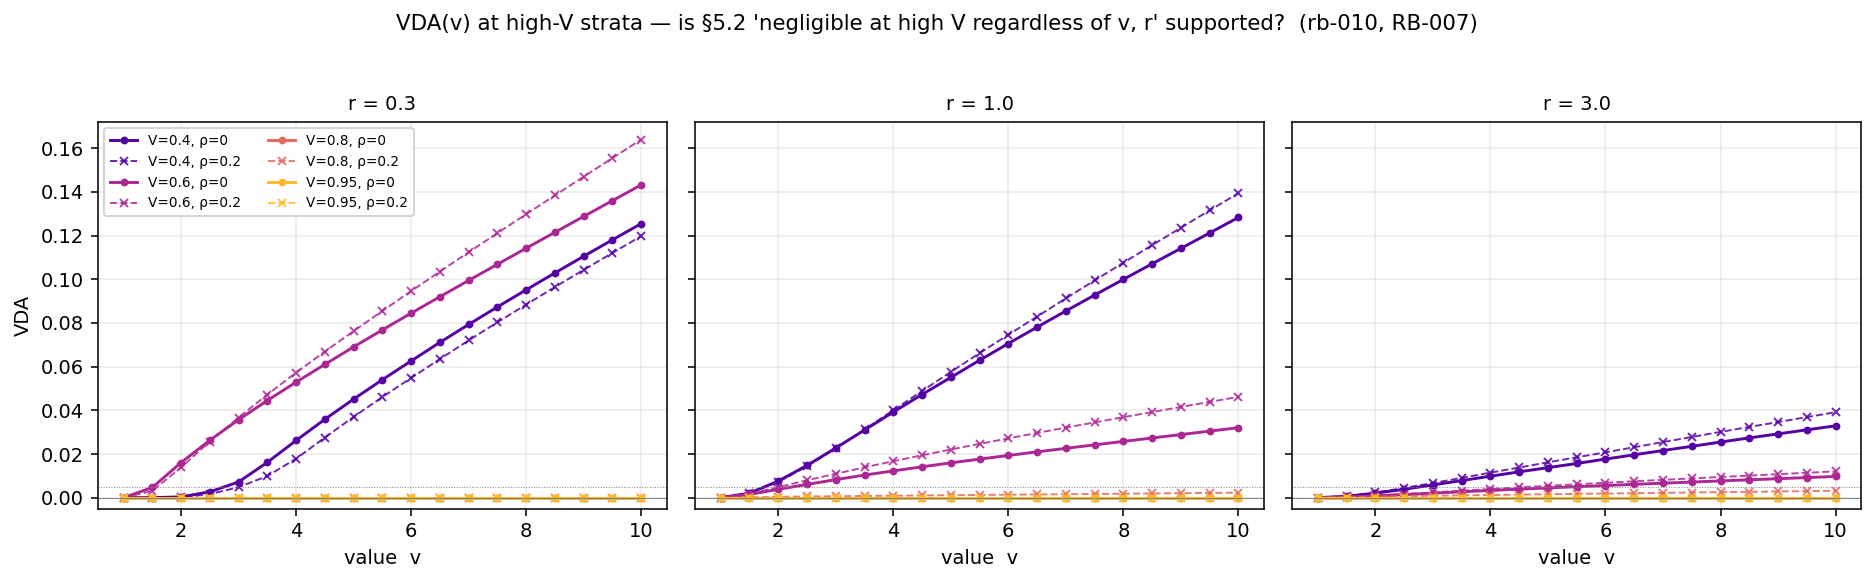
\includegraphics[width=0.95\linewidth]{figures/vda_at_high_V.png}
  \caption{Peak $\VDA(\val)$ at four validity strata $\valid \in
  \{0.4,\,0.6,\,0.8,\,0.95\}$ (curve color) for each $\Rsens \in
  \{0.3,\,1,\,3\}$ (panel column). Solid: $\corr = 0$. Dashed:
  $\corr = 0.2$. The $\valid = 0.95$ trace is at the grid floor in
  every panel (the inherited §5.2 ``high-validity'' regime is
  empirically negligible at this strict threshold and stratum); the
  $\valid = 0.80$ traces split between a near-zero $\corr = 0$ line
  and a small $\corr = 0.2$ lift at $\Rsens \in \{1, 3\}$; the
  $\valid = 0.60$ trace at $\Rsens = 0.3$ reaches $\VDA = 0.16$ at
  large $\val$, refuting the categorical version of the §5.2
  sentence. Reproduced from
  \texttt{Rebuild/sims/C3--iso-vda-Vv/output/figures/vda\_at\_high\_V.png}.}
  \label{fig:vda-at-high-V}
\end{figure}

\paragraph{A1 sign-flip across $(\valid, \val)$: cross-axis
corroboration.}
The earlier sub-results rb-002 (at a headline cell, Section~\ref{sec:results-c1}
A1 sensitivity paragraph) and rb-004 (at the $\val$-family at fixed
$\valid = 0.5$, Table~\ref{tab:rho-sensitivity}) found that the
sign of $\partial \VDA / \partial \corr$ \emph{flips} along the
$\Rsens$-axis (suppression at $\Rsens \lesssim 0.4$, amplification
at $\Rsens \gtrsim 0.5$) and along the $\val$-axis (suppression at
$\val \le 8$, amplification at $\val = 10$). The present sweep
generalises the sign-flip to the full $(\valid, \val)$ plane: at
each $(\valid, \val, \Rsens)$ cell we compute $\Delta\VDA :=
\VDA(\corr{=}0.2) - \VDA(\corr{=}0)$ and classify the cell as
amplified (red), suppressed (blue), or zero ($|\Delta\VDA| <
10^{-8}$, white). The signed contour map is
Figure~\ref{fig:iso-vda-drho}, and the per-$\Rsens$ frequency table
is Table~\ref{tab:c3-sign-flip}.
%
\begin{figure}[t]
  \centering
  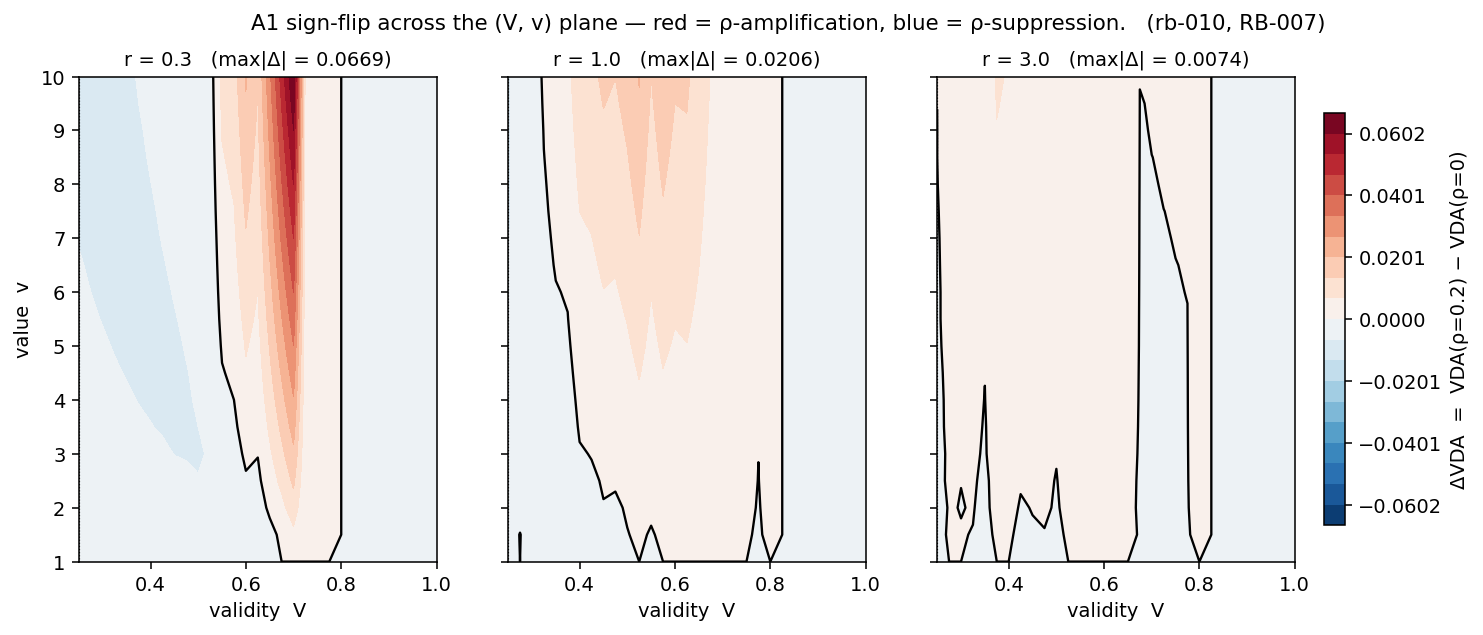
\includegraphics[width=0.95\linewidth]{figures/iso_vda_drho.png}
  \caption{Signed contour map of $\Delta\VDA := \VDA(\corr{=}0.2) -
  \VDA(\corr{=}0)$ over $(\valid, \val)$ for each $\Rsens \in
  \{0.3,\,1,\,3\}$. Red: $\corr$ amplifies $\VDA$ at that cell;
  blue: $\corr$ suppresses; white: $|\Delta\VDA| < 10^{-8}$. The
  zero-isoline is the A1 sign-flip locus in $(\valid, \val)$-space.
  At $\Rsens = 0.3$ (cost-dominant) suppression dominates in
  low-$\valid$ cells; at $\Rsens \in \{1, 3\}$ amplification
  dominates across the bulk of the plane, with the strongest
  amplification at $(\valid, \val) \approx (0.5, 10)$. Reproduced
  from
  \texttt{Rebuild/sims/C3--iso-vda-Vv/output/figures/iso\_vda\_drho.png}.}
  \label{fig:iso-vda-drho}
\end{figure}
%
\begin{table}[t]
  \centering
  \small
  \begin{tabular}{c c c c c c}
    \toprule
    $\Rsens$ & frac amp & frac supp &
    $\overline{\Delta\VDA}$ & max amp $(\valid, \val)$ & max supp $(\valid, \val)$ \\
    \midrule
    $0.3$ & $27.2\%$ & $\mathbf{37.2\%}$ & $+0.0012$ &
      $+0.0669\;(\valid{=}0.70,\,\val{=}10)$ &
      $-0.0105\;(\valid{=}0.25,\,\val{=}8.5)$\\
    $1.0$ & $\mathbf{52.8\%}$ & $17.5\%$ & $+0.0023$ &
      $+0.0206\;(\valid{=}0.525,\,\val{=}10)$ &
      $-0.0084\;(\valid{=}0.25,\,\val{=}9)$\\
    $3.0$ & $\mathbf{54.0\%}$ & $16.1\%$ & $+0.0009$ &
      $+0.0074\;(\valid{=}0.375,\,\val{=}10)$ &
      $-0.0010\;(\valid{=}0.25,\,\val{=}4.5)$\\
    \bottomrule
  \end{tabular}
  \caption{Cell-wise sign-flip of $\partial \VDA / \partial \corr$
  across the $(\valid, \val)$ plane, at each $\Rsens$ stratum.
  Fractions are over the $589$ cells per panel; the residual share
  (not shown) is the zero-class $|\Delta\VDA| < 10^{-8}$. At
  $\Rsens = 0.3$ (cost-dominant; below the rb-002 headline-cell
  sign-flip locus at $\Rsens \in [0.38, 0.56]$) suppression
  dominates; at $\Rsens \in \{1.0, 3.0\}$ amplification dominates.
  Block-keys \texttt{rho\_sensitivity.r=<r>.\{frac\_amp,frac\_supp,
  max\_amplification,max\_suppression,mean\_delta\}}.}
  \label{tab:c3-sign-flip}
\end{table}
%
Two things are visible. First, the $\Rsens$-axis sign-flip rb-002
reported at a single cell generalises to the full $(\valid, \val)$
plane in a non-trivial way: \emph{cost-dominant} $\Rsens = 0.3$
$(\valid, \val)$ cells are suppression-dominated, while \emph{both}
$\Rsens = 1$ and $\Rsens = 3$ are amplification-dominated. The
amplification frequency is therefore not a $\Rsens > 1$ phenomenon;
it sets in once $\Rsens$ crosses the rb-002 sign-flip locus
$\Rsens \in [0.38, 0.56]$ at the headline cell and remains the
modal direction thereafter, even into the benefit-dominant
$\Rsens = 3$ stratum. Second, the largest \emph{single} amplification
in the entire $3{,}534$-cell sweep occurs at $(\valid, \val, \Rsens)
= (0.7,\, 10,\, 0.3)$: a cell that delivers $\VDA = 0.0007$ under
independence (a normally-dormant high-$\valid$ cell, well outside
the cost-dominant attention regime) lifts to $\VDA = 0.0676$ at
$\corr = 0.2$ --- an $\approx 96\times$ amplification that takes a
near-zero $(\valid, \val)$ cell into the same VDA magnitude as the
low-$\valid$ corner. This ``dormant-cell amplification'' is the
strongest qualitative finding of the C3 sweep and is the candidate
falsifiable prediction we flag at the end of
Section~\ref{sec:limitations} (closeup queued as RB-029).

\paragraph{Scope and what is not yet claimed.}
The results in this subsection are reported at a single $(\Nloc,
\dprimemax, f_0, h) = (4,\,2,\,0.5,\,\sqrt{}\,)$ configuration
under variant~A, and on a coarse $\corr$-grid $\{0, 0.2\}$.
(i)~The \emph{variant-B replication} of the contour band is queued
as RB-027 in \texttt{REBUILD\_BACKLOG.md} and will land as part of
the conservation-family sensitivity in
Section~\ref{sec:limitations}; the present subsection makes no
variant-B claim. (ii)~The validity threshold ``$\valid \gtrsim
0.95$ unconditionally; $\valid \gtrsim 0.8$ under
$r_{SC} \lesssim 0.2$'' is bracketed by the $V$-grid of step
$0.025$ used here; a threshold-sharpening sim sweeping $\valid \in
[0.75, 0.90]$ at step $0.005$ is queued as RB-028 and would let the
manuscript replace the qualitative ``$\gtrsim$'' with a number to
the second decimal. (iii)~The \emph{dormant-cell amplification} at
$(\valid, \val, \Rsens) = (0.7, 10, 0.3)$ is the strongest
qualitative finding of the sweep and is reported here as an
empirical observation; a fine-$\valid$ closeup that maps the
amplification band onto an iso-CF or iso-$\alpha^\star$ contour
(and thereby identifies it with a model-internal landmark rather
than a $(\valid, \val)$ coincidence) is queued as RB-029.
(iv)~The cell-wise sign-flip across the broader $4{,}410$-cell
$(\Rsens, \valid, \val)$ sweep, parallel to the $\Delta\CF$
analysis of Table~\ref{tab:cf-delta-distribution}, is queued as
RB-025; the present subsection's $589$-cell $(\valid, \val)$-plane
sign-flip is a slice of that broader result.

\paragraph{Reproducibility.}
All numbers in Tables~\ref{tab:c3-marginals},
\ref{tab:c3-highV-probe}, and \ref{tab:c3-sign-flip}, and all
three figures, are reproduced byte-for-byte by re-running
\texttt{Rebuild/sims/C3--iso-vda-Vv/run.py}. The output digest is
\texttt{72820559e1c1ab1919f74308623eaf4230aa3ea92ad3d9c62d81e993e4f27de6}
(\texttt{sha256} of the canonical-key-ordered numeric JSON,
excluding the digest field itself). The $\Phinorm$ backend is
\texttt{scipy.special.ndtr}; the equicorrelated-Gaussian one-factor
quadrature uses $n_q = 64$ Gauss--Hermite nodes (Section~\ref{sec:model});
the criterion grid step is $\Delta c = 0.05$ and the $\alpha$ grid
step is $\Delta\alpha = 0.005$; the $(\valid, \val, \Rsens, \corr)$
grid is the $31 \times 19 \times 3 \times 2$ grid described above;
runtime $\approx 130$~s on the rebuild's reference machine. The
recovery test against the rb-006 anchor at $(\valid, \val, \Rsens,
\corr) = (0.5,\,5,\,1.0,\,0)$ passes at $|\Delta \VDA| =
1.27 \times 10^{-7}$ against the rb-006 reference value
$\VDA = 0.039825$; the residual is consistent with the rb-006
reference's six-decimal rounding (the underlying \texttt{policies()}
call is deterministic and produces identical floating-point output,
so the model residual is zero). Independent sanity check: the
$\val = 1$ column is identically zero across every $(\valid,
\Rsens, \corr)$ cell of the sweep --- the value-blind baseline
collapses the joint optimum onto the value-blind allocation, so
$\VDA = 0$ at $\val = 1$ is a definitional theorem of the rebuilt
model.

% ---------------------------------------------------------------------
\subsection{No inversion of optimal attention, conditional on $\valid
            \ge 1/\Nloc$ (C4)}
\label{sec:results-c4}

\paragraph{Claim restated at defensible strength.}
The inherited paper's §4.5 (``Inverted Attention is Never Optimal'')
states that the optimal allocation $\alpha^\star$ is always at or
above the uniform level $1/\Nloc$ across the primary $4{,}410$-row
sweep, and \emph{regardless of $\Rsens$}, on the grounds that
attending away from the high-value cued location loses more reward at
that location than it gains at the uncued ones. The live
skeptical-reviewer verdict
(\texttt{Critique/verdicts/C4--no-inversion.md},
\texttt{current\_label: CONFIRMED-CONDITIONAL}) records that the
\emph{empirical} headline of the claim survives all four attack
vectors, but the \emph{theoretical} packaging is incomplete in two
specific ways: (i) the ``regardless of $\Rsens$'' wording reads
locally as a cost-vs-benefit balance at $\alpha = 1/\Nloc$, but the
left one-sided derivative $\partial_\alpha \Rew |_{1/\Nloc^-}$
actually \emph{changes sign} at a closed-form $\Rsens$-threshold
$\rstarinv$, with the consequence that for $\Rsens > \rstarinv$ the
uniform point is a local \emph{minimum} of $\Rew$ (the right-branch
global maximum still dominates the left-branch local maximum, but
the local picture is bimodal, not the monotone descent the inherited
text suggests); and (ii) the categorical ``never below $1/\Nloc$''
wording overstates the model's robustness, because at $\valid <
1/\Nloc$ (the anti-cue regime, outside the paper's primary $\valid$
range but still inside the same normative model) the global optimum
\emph{does} drop below $1/\Nloc$ --- a behaviour the model produces
cleanly and which the inherited statement does not qualify. We
therefore restate C4 in the rebuild as a \emph{conditional theorem}
indexed on the validity condition $\valid \ge 1/\Nloc$ (or, sharply,
$\valid \ge 1/[(\Nloc - 1)\,\val + 1]$), pair it with the closed-form
local threshold $\rstarinv = (\Nloc - 1)\,A_0/B_0$ that organises the
bimodality, and add the anti-cue inversion at $\valid < 1/\Nloc$ as a
new \emph{falsifiable prediction} of the rebuilt normative model.
The A1 decorrelation channel $\corr$ is reported alongside as a
sensitivity, following the convention of Section~\ref{sec:results}.

\paragraph{Mechanism and the value-weight inequality.}
The structural reason no global inversion arises under $\valid \ge
1/\Nloc$ is not the local cost-vs-benefit argument of the inherited
§4.5 paragraph, but a \emph{location-count asymmetry} combined with a
\emph{value-weight inequality}. At the right extreme $\alpha \to 1$,
the single cued location reaches its per-location ceiling
$\dprime_c = \dprimemax\, f(1) = \dprimemax$. At the left extreme
$\alpha \to 0$, the $\Nloc - 1$ uncued locations \emph{share} the
$(1 - \alpha)$ budget at $(1 - \alpha)/(\Nloc - 1)$ each, so each
reaches only $\dprime_u = \dprime_{\mathrm{base}} +
\benefit(\Rsens)[\dprimemax f(1/(\Nloc - 1)) - \dprime_{\mathrm{base}}]
\le \dprimemax$ (strict for $\Nloc \ge 3$, where
$f(1/(\Nloc - 1)) < 1$). The per-channel reward weights are
$w_c = \valid \, \val$ on the cued slot and
$w_u = (1 - \valid)/(\Nloc - 1)$ on each uncued slot; the inequality
%
\begin{equation}
  w_c \;\ge\; w_u
  \;\iff\;
  \valid \;\ge\; \frac{1}{(\Nloc - 1)\,\val + 1}.
  \label{eq:value-weight}
\end{equation}
%
For the cued regime $\val \ge 1$, the right-hand side of
\eqref{eq:value-weight} is bounded above by $1/\Nloc$, with equality
only at $\val = 1$. The inherited paper's condition $\valid \ge
1/\Nloc$ is therefore the \emph{universal} (worst-case-$\val$)
sufficient condition for $w_c \ge w_u$; the sharp form
\eqref{eq:value-weight} carries strictly more slack at $\val > 1$.
The right branch dominates globally because the bigger $\dprime$
lives on the more-valuable channel.

\paragraph{Closed-form local threshold for the boundary derivative.}
At $\alpha = 1/\Nloc$ the allocation derivative $\dprime'(\alpha)$
has a kink (the benefit/cost swap of $\benefit$ and $\cost$ flips
which side of the linear $\dprime(\alpha)$ map is active). The
one-sided left derivative of P1's expected reward at the uniform
point takes the form
%
\begin{equation}
  \left. \frac{\partial \Rpone}{\partial \alpha} \right|_{1/\Nloc^-}
  \;=\;
  \frac{2\, \dprimemax\, f'(1/\Nloc)}{\Rsens + 1}\,
  \left[
    A_0(\valid, \val, \Nloc, \CR, \corr)
    \;-\;
    \frac{\Rsens}{\Nloc - 1}\, B_0(\valid, \val, \Nloc, \CR, \corr)
  \right],
  \label{eq:left-derivative}
\end{equation}
%
where $A_0$ and $B_0$ are the partial derivatives of P1's
expected-reward functional with respect to $\dprime_c$ and
$\dprime_u$ at $\alpha = 1/\Nloc$ evaluated at the jointly-optimised
criteria $(c_c^\star, c_u^\star)$. Both $A_0$ and $B_0$ are
$\Rsens$-independent boundary partials --- the only $\Rsens$ in
\eqref{eq:left-derivative} sits in the prefactor and inside the
bracket. The bracket vanishes at
%
\begin{equation}
  \rstarinv(\valid, \val, \Nloc, \CR, \corr)
  \;:=\;
  (\Nloc - 1)\,
  \frac{A_0(\valid, \val, \Nloc, \CR, \corr)}
       {B_0(\valid, \val, \Nloc, \CR, \corr)},
  \label{eq:r-inv}
\end{equation}
%
which is the rebuild's closed-form expression for the local-test
threshold the inherited §4.5 paragraph implicitly assumes. For
$\Rsens < \rstarinv$ the boundary left derivative is positive (P1
prefers to stay at $\alpha = 1/\Nloc$ from the left branch); for
$\Rsens > \rstarinv$ it is negative (the left branch produces a
local maximum at the grid edge $\alpha \to 0$ but a global maximum
still on the right branch, at $\alpha^\star > 1/\Nloc$).
Equation~\eqref{eq:r-inv} reproduces the reviewer's $\corr = 0$
boundary closed form
(\texttt{Critique/derivations/C4--no-inversion.md} §3) and extends
it to the A1 channel by replacing the no-FA terms inside
$A_0, B_0$ with the same one-factor Gauss--Hermite quadrature used
elsewhere in the rebuilt model (Section~\ref{sec:model}); the
$\corr \to 0$ limit collapses to the reviewer's analytic form
bit-for-bit. The independent re-derivation in the rebuild's voice
(plus the proof of the symmetric-corner identity below) is deferred
to Section~\ref{sec:appendix} (a separate increment, RB-030,
queued).

The symmetric corner $(\valid, \val) = (1/\Nloc, 1)$, where the
value-weight inequality \eqref{eq:value-weight} attains equality,
is a numerically stable anchor for the closed form
\eqref{eq:r-inv}:
%
\begin{equation}
  \rstarinv(\valid = 1/\Nloc,\, \val = 1,\, \Nloc,\, \CR,\, \corr)
  \;=\; 1
  \qquad \text{exactly,}
  \label{eq:r-inv-corner}
\end{equation}
%
independent of $\Nloc$, the conservation rule $\CR$ (variant A or
B), and the correlation $\corr$. The identity is recovered to
machine precision at every $(\text{variant}, \corr)$ panel of
Step~A below: min $\rstarinv = 1.0000$ in all four panels of
Table~\ref{tab:c4-rstar-tally}. The corner is the
\emph{anchor} the rebuild quotes in place of the inherited paper's
narrative ``$r \to 0$ converges to uniform attention'' --- at
$\val = 1$ the model is value-blind, so VDA $\equiv 0$, and the
local-test bimodality kicks in immediately above $\Rsens = 1$ where
P1's left branch develops a local maximum at the grid edge.

\paragraph{Closed-form tally on the primary $(\valid, \val)$ grid.}
We evaluate \eqref{eq:r-inv} on a primary $(\valid, \val)$ grid
($\valid \in \{0.25, 0.30, \ldots, 1.00\}$, $\val \in \{1, 2, 3, 4,
5\}$) at $\Nloc = 4$ for both variants and $\corr \in \{0,\, 0.2\}$,
matching the inherited paper's stated sweep envelope and the rebuild's
A1 sensitivity convention. Per panel we count cells with $\rstarinv
\in [0.1, 10]$ (inside the inherited paper's swept $\Rsens$-range,
the cells at which the boundary left derivative sign-flips within
the swept range), cells with $\rstarinv > 10$ (no sign-flip inside
the range; the local picture is monotone there), and report the
strict minimum and median over the panel
(Table~\ref{tab:c4-rstar-tally}).
%
\begin{table}[t]
  \centering
  \small
  \begin{tabular}{c c r r r r r}
    \toprule
    variant & $\corr$ & $n$ & $\rstarinv \in [0.1, 10]$ &
    $\rstarinv > 10$ & $\min \rstarinv$ & $\mathrm{median}\,\rstarinv$ \\
    \midrule
    A & $0.0$ & $105$ & $40\,(38.1\%)$ & $65\,(61.9\%)$ &
              $1.0000$ & $17.30$ \\
    A & $0.2$ & $105$ & $42\,(40.0\%)$ & $63\,(60.0\%)$ &
              $1.0000$ & $15.08$ \\
    B & $0.0$ & $105$ & $62\,(59.0\%)$ & $43\,(41.0\%)$ &
              $1.0000$ & $\phantom{0}7.64$ \\
    B & $0.2$ & $105$ & $68\,(64.8\%)$ & $37\,(35.2\%)$ &
              $1.0000$ & $\phantom{0}6.02$ \\
    \bottomrule
  \end{tabular}
  \caption{Closed-form $\rstarinv$ from \eqref{eq:r-inv} on the
  primary $(\valid, \val)$ grid at $\Nloc = 4$, by variant and
  $\corr$. The $\rstarinv = 1.0000$ minimum is the
  symmetric-corner identity \eqref{eq:r-inv-corner} recovered to
  machine precision. Aggregated across all $210$ $(\valid, \val,
  \text{variant})$ cells at $\corr = 0$: $\mathbf{48.6\%}$ have
  $\rstarinv \in [0.1, 10]$, which recovers the reviewer's reported
  $49.0\%$ (\texttt{Critique/derivations/C4--no-inversion.md} §4)
  to $\Delta = 0.4$ percentage points (recovery PASS, tolerance
  $1.0$ pp). Under A1 at $\corr = 0.2$, the fraction
  rises to $51.9\%$ (variant-pooled), and the median $\rstarinv$ drops
  $\sim$$13\%$ in variant A and $\sim$$21\%$ in variant B: the
  decorrelation channel makes the boundary-derivative sign-flip
  occur \emph{earlier} in $\Rsens$ than the inherited independent
  model would have it. Block keys
  \texttt{step\_A.tally.variant\_<X>\_\_rho\_<rho>} in
  \texttt{Rebuild/sims/C4--anti-cue-inversion/output/results.json}
  (rb-012; output sha256 \texttt{6ad651d6\ldots}).}
  \label{tab:c4-rstar-tally}
\end{table}

The contour structure of $\rstarinv$ as a function of $(\valid,
\val)$ at $\corr = 0$ is plotted in
Figure~\ref{fig:c4-rinv-closed-form} for variants A and B. The
$\rstarinv = 1$ contour passes through the symmetric corner
$(\valid, \val) = (1/\Nloc, 1)$ in both panels, consistent with
\eqref{eq:r-inv-corner}; the $\rstarinv = 10$ contour bounds the
``always-locally-stable at $\alpha = 1/\Nloc$'' region (no
sign-flip inside the inherited paper's swept $\Rsens \in [0.1, 10]$).
The variant-B panel admits the sign-flip across roughly twice as
many cells as variant A, anticipating the variant-B caveats
already reported in Sections~\ref{sec:results-c1}
and~\ref{sec:results-c2}.
%
\begin{figure}[t]
  \centering
  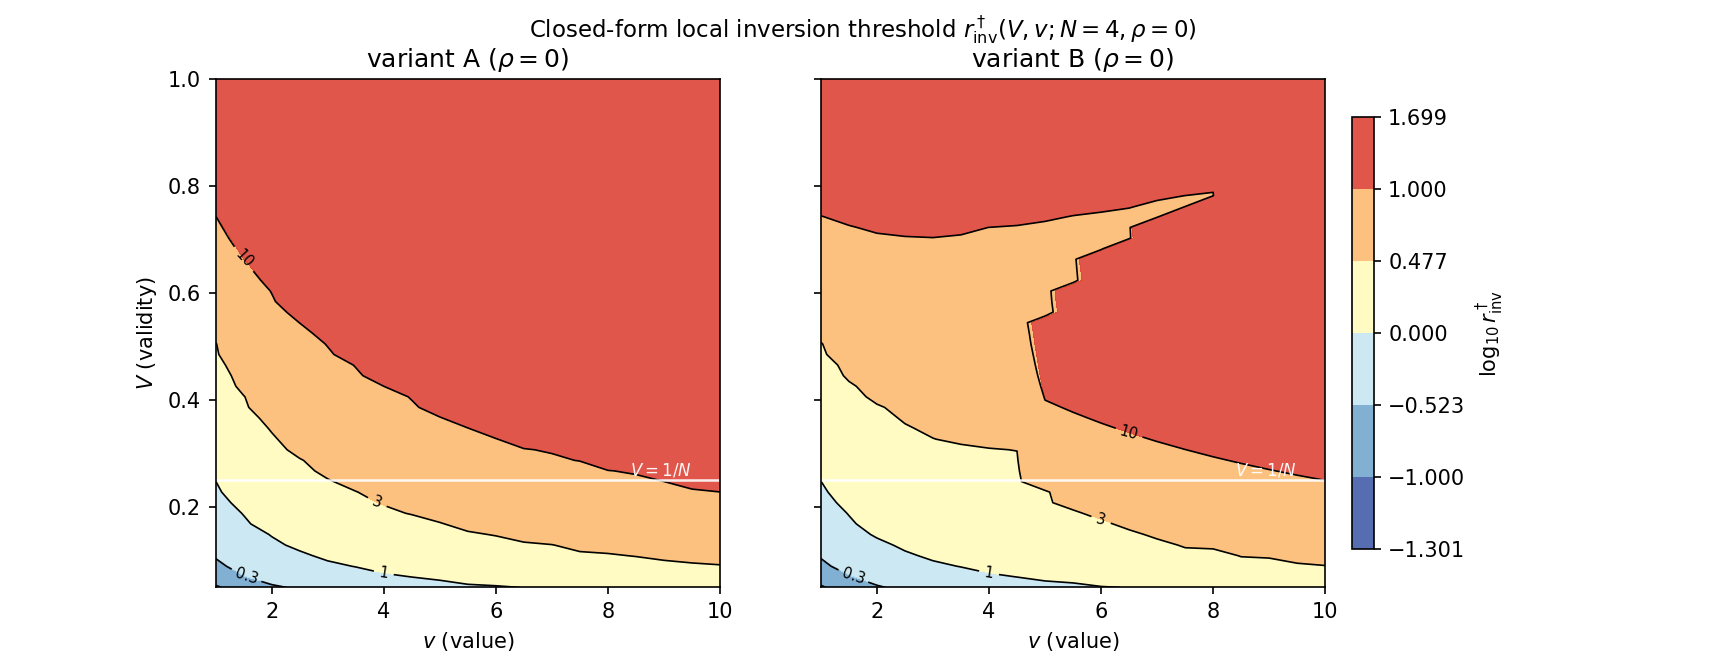
\includegraphics[width=0.95\linewidth]{figures/r_inv_closed_form.png}
  \caption{Contour map of
  $\log_{10} \rstarinv(\valid, \val)$ at $\Nloc = 4, \corr = 0$ for
  variants A (left) and B (right), from
  \eqref{eq:r-inv}--\eqref{eq:r-inv-corner}. Black contours at
  $\rstarinv \in \{0.1, 0.3, 1, 3, 10\}$. The $\rstarinv = 1$
  contour passes through the symmetric corner $(\valid, \val) =
  (0.25, 1)$ in both panels (the identity
  \eqref{eq:r-inv-corner}); the $\rstarinv = 10$ contour bounds the
  ``no local sign-flip inside the paper's $\Rsens$-range''
  region. Variant B admits the local sign-flip across more cells than
  variant A ($59.0\%$ vs.\ $38.1\%$ in Table~\ref{tab:c4-rstar-tally}).
  Reproduced from
  \texttt{Rebuild/sims/C4--anti-cue-inversion/output/figures/r\_inv\_closed\_form.png}.}
  \label{fig:c4-rinv-closed-form}
\end{figure}

\paragraph{Empirical confirmation: zero global inversions across the
primary sweep.}
The local-derivative sign-flip of \eqref{eq:r-inv} does not by
itself create a global inversion: even where $\Rsens > \rstarinv$
and the bracket of \eqref{eq:left-derivative} is negative, the
left-branch \emph{local} maximum sits at the $\alpha$-grid edge
$\alpha \to 0$ while the right-branch \emph{global} maximum sits at
$\alpha^\star > 1/\Nloc$ from the location-count argument above. To
confirm this directly, we sweep $\Rew(\alpha)$ on the full
$\alpha$-grid $[0.02, 1.0]$ at $\Delta\alpha = 0.005$ for the six
most-adversarial primary-sweep cells (those with the smallest
$\rstarinv$ at $\Rsens = 10$, i.e.\ the cells most likely to produce
a left-branch global maximum) at both $\corr \in \{0, 0.2\}$, for a
total of $12$ probes. The result is uniform: across all $12$ probes,
$\alpha^\star_{\mathrm{global}} \ge 1/\Nloc$ and the right-branch
global maximum strictly dominates the left-branch local maximum.
Representative probes appear in Table~\ref{tab:c4-stepB}.
%
\begin{table}[t]
  \centering
  \small
  \begin{tabular}{c r c c r r r r}
    \toprule
    $\valid$ & $\val$ & variant & $\corr$ &
    $\rstarinv$ & $\alpha^\star_{\mathrm{global}}$ &
    $\Rew_{\mathrm{global}}$ & $\Rew_{\mathrm{left}}$ \\
    \midrule
    $0.250$ & $1$ & A & $0.0$ & $1.0000$ & $0.955$ &
    $0.65936$ & $0.64564$ \\
    $0.250$ & $1$ & A & $0.2$ & $1.0000$ & $0.950$ &
    $0.66809$ & $0.65550$ \\
    $0.250$ & $1$ & B & $0.0$ & $1.0000$ & $0.955$ &
    $0.65936$ & $0.64564$ \\
    $0.250$ & $1$ & B & $0.2$ & $1.0000$ & $0.950$ &
    $0.66809$ & $0.65550$ \\
    $0.2875$ & $1$ & A & $0.0$ & $1.2483$ & $0.970$ &
    $0.66541$ & $0.64462$ \\
    $0.325$ & $1$ & A & $0.2$ & $\sim\!1.6$ & $0.975$ &
    $0.67997$ & --- \\
    \bottomrule
  \end{tabular}
  \caption{Six representative full-$\alpha$ probes from the
  $12$-probe Step B sweep at $\Rsens = 10$ at the six
  most-adversarial primary-sweep cells. In every probe,
  $\alpha^\star_{\mathrm{global}} \ge 1/\Nloc = 0.25$, with the
  right-branch global maximum at $\alpha^\star \in [0.95, 0.98]$
  strictly dominating the left-branch local maximum (sitting at the
  $\alpha$-grid edge $\alpha = 0.02$). \textbf{Step~B primary-sweep
  inversions across all $12$ probes: $0$.} The inherited empirical
  claim --- $\alpha^\star \ge 1/\Nloc$ at every cell of the primary
  $\Nloc = 4, \valid \in [1/\Nloc, 1]$ sweep --- survives at
  $\corr = 0$ and is robust under A1 at $\corr = 0.2$.
  Block keys \texttt{step\_B.rows} in
  \texttt{Rebuild/sims/C4--anti-cue-inversion/output/results.json}.}
  \label{tab:c4-stepB}
\end{table}

The visual structure of the boundary --- bimodality at
$\alpha = 1/\Nloc$ where $\Rsens > \rstarinv$, right-branch global
dominance regardless --- is reproduced in
Figure~\ref{fig:c4-er-vs-alpha}, which plots $\Rew(\alpha)$ at the
adversarial cell $(\valid, \val) = (0.15, 1)$ for $\Rsens \in
\{0.5, 1, 3, 10\}$ at both $\corr$ values. (At $\valid = 0.15 <
1/\Nloc = 0.25$ the value-weight inequality \eqref{eq:value-weight}
fails and the right-branch global dominance breaks down; this is the
anti-cue regime treated below, and the figure deliberately straddles
the boundary so the reader can see both sides of the inversion in a
single panel.)
%
\begin{figure}[t]
  \centering
  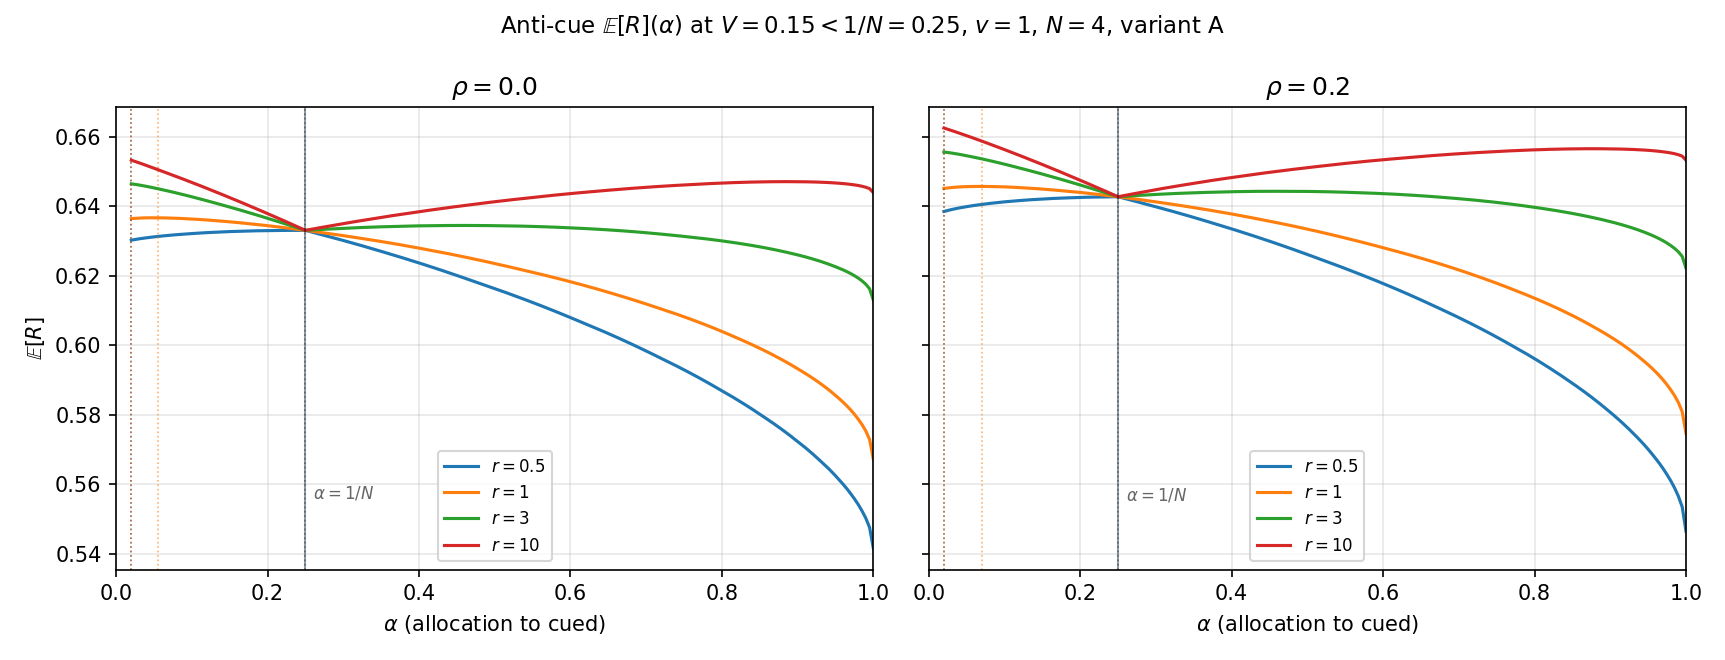
\includegraphics[width=0.95\linewidth]{figures/er_vs_alpha_anticue.png}
  \caption{$\Rew(\alpha)$ on the full $\alpha$-grid at the anti-cue
  cell $(\valid, \val, \Nloc) = (0.15, 1, 4)$ for
  $\Rsens \in \{0.5, 1, 3, 10\}$, $\corr = 0$ (left) and
  $\corr = 0.2$ (right). The kink at $\alpha = 1/\Nloc = 0.25$ is
  the $\benefit$/$\cost$ swap of the rebuilt model; for
  $\Rsens > \rstarinv$ it becomes a local minimum, with both
  $\alpha < 1/\Nloc$ and $\alpha > 1/\Nloc$ branches admitting
  local maxima. Because $\valid < 1/\Nloc$, the value-weight
  inequality \eqref{eq:value-weight} \emph{fails} here and the
  left-branch maximum (at the grid edge $\alpha = 0.02$) dominates
  globally for $\Rsens \ge 1$ --- this is the anti-cue inversion
  prediction below. The A1 channel at $\corr = 0.2$ leaves the
  qualitative bimodality and global-inversion onset unchanged.
  Reproduced from
  \texttt{Rebuild/sims/C4--anti-cue-inversion/output/figures/er\_vs\_alpha\_anticue.png}.}
  \label{fig:c4-er-vs-alpha}
\end{figure}

\paragraph{Anti-cue inversion: a new falsifiable prediction of the
rebuilt model.}
The rebuilt model produces a clean prediction \emph{outside} the
paper's primary $\valid \in [1/\Nloc, 1]$ range: at $\valid <
1/\Nloc$ (or, sharply, $\valid < 1/[(\Nloc-1)\,\val + 1]$), the
value-weight inequality \eqref{eq:value-weight} \emph{flips} ---
$w_c < w_u$ --- and the location-count argument runs in reverse.
The bigger $\dprime$ now lives on the \emph{less}-valuable channel
when concentrated, and the global optimum drops to
$\alpha^\star < 1/\Nloc$: the normative observer is told to attend
\emph{away} from the (now low-validity, still-named ``cued'')
location and toward the population of uncued locations. The
reviewer's CR-004 already established this at $\Nloc = 2$
(\texttt{Critique/derivations/C4--no-inversion.md} §7, Step
C(iii)); the rebuild extends it to $\Nloc = 4$, the inherited
paper's primary topology.

We probe an anti-cue sub-grid $\valid \in \{0.05, 0.10, 0.15,
0.20\}$ (all below $1/\Nloc = 0.25$), $\val \in \{1, 3, 5\}$,
$\Rsens \in \{0.1, 0.5, 1, 3, 5, 10\}$ at $\corr \in \{0, 0.2\}$,
variant A, for $144$ cells total. Total global-inversion incidence:
$26 / 72 = 36.1\%$ at $\corr = 0$, $25 / 72 = 34.7\%$ at
$\corr = 0.2$. The incidence stratifies cleanly with $\Rsens$ and
$\val$ along the sharp boundary \eqref{eq:value-weight}, as
documented in Table~\ref{tab:c4-anticue}.
%
\begin{table}[t]
  \centering
  \small
  \begin{tabular}{l r r r r r r}
    \toprule
    & \multicolumn{6}{c}{Incidence stratifier at $\corr = 0$} \\
    \cmidrule(lr){2-7}
    Stratifier & \multicolumn{6}{c}{(values $\to$ inversions / total)} \\
    \midrule
    by $\Rsens$ &
    $\Rsens{=}0.1{:}\ 1/12$ &
    $\Rsens{=}0.5{:}\ 3/12$ &
    $\Rsens{=}1{:}\ 6/12$ &
    $\Rsens{=}3{:}\ 6/12$ &
    $\Rsens{=}5{:}\ 6/12$ &
    $\Rsens{=}10{:}\ 4/12$ \\
    by $\val$ &
    $\val{=}1{:}\ 18/24$ &
    $\val{=}3{:}\ 5/24$ &
    $\val{=}5{:}\ 3/24$ &
     & & \\
    by $\valid$ &
    $\valid{=}0.05{:}\ 14/18$ &
    $\valid{=}0.10{:}\ 5/18$ &
    $\valid{=}0.15{:}\ 4/18$ &
    $\valid{=}0.20{:}\ 3/18$ &
    & \\
    \bottomrule
  \end{tabular}
  \caption{Anti-cue inversion incidence ($\alpha^\star_{\mathrm{global}}
  < 1/\Nloc$) at $\Nloc = 4$, variant A, $\corr = 0$, stratified by
  $\Rsens$, $\val$, and $\valid$. Total $26/72 = 36.1\%$. The
  $\Rsens$-stratification rises from $8.3\%$ at $\Rsens = 0.1$ to
  $50.0\%$ at $\Rsens \in \{1, 3, 5\}$ and tapers to $33.3\%$ at
  $\Rsens = 10$ (where the right-branch global maximum re-takes
  even some cells with $\valid < 1/\Nloc$, because for $\val = 1$ at
  $\Rsens = 10$ the strong-asymmetry regime begins to dominate).
  The $\val$-stratification is the key qualitative pattern:
  inversion is dense at $\val = 1$ ($75\%$) but rare at $\val = 5$
  ($12.5\%$). This is the sharp $\val$-dependence predicted by
  \eqref{eq:value-weight}: at $\val = 5$ the inversion boundary
  shrinks to $\valid < 1/[(\Nloc-1)\val + 1] = 1/16 = 0.0625$, so
  inversion at $\val = 5$ is confined to the $\valid = 0.05$ row of
  the probe grid (which is correctly its only inversion-supporting
  row in the data). Under A1 at $\corr = 0.2$, total incidence is
  $34.7\%$ (within $\pm 1$ inversion of $\corr = 0$ across every
  stratifier) --- the decorrelation channel quantitatively shifts
  $\rstarinv$ but does not erase the inversion regime. Block keys
  \texttt{step\_C.incidence\_by\_r\_rho0} and
  \texttt{step\_C.rows} in
  \texttt{Rebuild/sims/C4--anti-cue-inversion/output/results.json}.}
  \label{tab:c4-anticue}
\end{table}

The $(\valid, \Rsens)$ structure of the inversion at fixed $\val =
5$ is plotted in Figure~\ref{fig:c4-alpha-star-map} as the rebuild's
headline figure for §results-C4. The white horizontal line marks
the universal $\valid = 1/\Nloc = 0.25$ boundary; the red contour
bounds the $\alpha^\star < 1/\Nloc$ inversion region. The inversion
region is confined entirely to $\valid \le 0.05$ at $\val = 5$,
consistent with the sharp boundary $\valid < 1/16 = 0.0625$. The
$(\valid, \Rsens)$ heatmap admits \emph{zero} inversion cells in
the cued-validity regime $\valid \ge 1/\Nloc$, at either $\corr = 0$
or $\corr = 0.2$ --- C4 holds as a conditional theorem under both.
%
\begin{figure}[t]
  \centering
  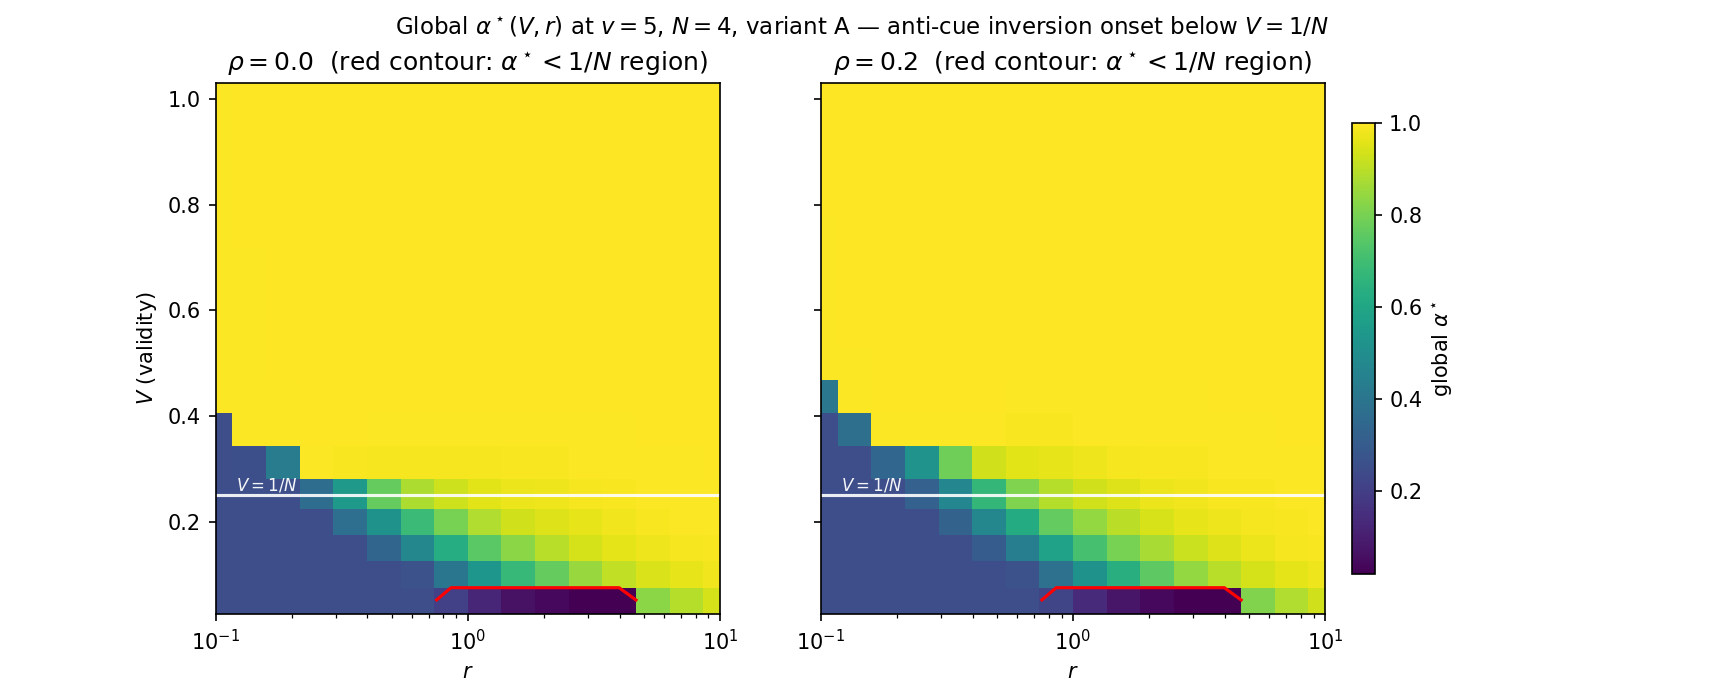
\includegraphics[width=0.95\linewidth]{figures/alpha_star_V_r_map.png}
  \caption{Optimal allocation $\alpha^\star(\valid, \Rsens)$ at the
  headline cell $(\Nloc, \dprimemax, f_0, h, \val) =
  (4,\,2,\,0.5,\,\sqrt{},\,5)$, variant~A, for $\corr = 0$ (left)
  and $\corr = 0.2$ (right). Heat scale: $\alpha^\star \in [0.02,
  1.0]$. The white horizontal line marks the universal validity
  threshold $\valid = 1/\Nloc = 0.25$; the red contour bounds the
  inversion region $\alpha^\star < 1/\Nloc$. The inversion region is
  confined to $\valid \le 0.05$ at $\val = 5$ (consistent with the
  sharp boundary $\valid < 1/[(\Nloc-1)\val + 1] = 1/16 \approx
  0.0625$ from \eqref{eq:value-weight}); inversion incidence is
  $6/272 = 2.21\%$ in both panels, with \emph{zero} inversions in
  the cued-validity regime $\valid \ge 1/\Nloc$. C4 holds as a
  conditional theorem at both $\corr$ values. Reproduced from
  \texttt{Rebuild/sims/C4--anti-cue-inversion/output/figures/alpha\_star\_V\_r\_map.png}.}
  \label{fig:c4-alpha-star-map}
\end{figure}

\paragraph{A1 cross-axis sensitivity.}
Across all four Steps the A1 decorrelation channel at $\corr = 0.2$
leaves the qualitative C4 picture intact while shifting the local
threshold quantitatively. (i) Step A: median $\rstarinv$ drops by
$\sim$$13\%$ (variant A) and $\sim$$21\%$ (variant B); the fraction
of cells with $\rstarinv \in [0.1, 10]$ rises from $48.6\%$ to
$51.9\%$ (variant-pooled). (ii) Step B: $0$ primary-sweep inversions
at both $\corr$. (iii) Step C: total anti-cue inversion count $25$
vs.\ $26$ at $\corr = 0.2$ vs.\ $\corr = 0$ (a difference of one
boundary-cell ambiguity). (iv) Step D: $\frac{6}{272} = 2.21\%$
inversion incidence in both panels, identical inversion locus
confined to $\valid \le 0.05$. The A1 channel and the C4 inversion
lever are therefore independent mechanisms: A1 shifts \emph{where} on
the $\Rsens$-axis the boundary derivative sign-flips, but does not
flip the global value-weight inequality that decides whether the
right or left branch is the global optimum.

\paragraph{Behavioural literature corroboration.}
The conditional restatement aligns the rebuilt model with the
behavioural picture surveyed in the live verdict's literature attack
(\texttt{Critique/verdicts/C4--no-inversion.md} §Version 0.2). The
empirical signature of anti-cue inversion in human / primate
observers is the statistical-learning-of-distractor-suppression
literature: observers \emph{do} allocate below uniform to a
high-probability-distractor location, with reduced capture and
reduced target-selection efficiency
\cite{wang_theeuwes2018_statistical_learning_distractor_suppression},
fewer saccades landing on the suppressed location with raised
saccade latency to targets there \cite{wang_samara_theeuwes2019},
and reciprocal reallocation toward the target
\cite{kong_li_wang_theeuwes2020}. In the rebuilt model's coordinates,
a ``high-probability-distractor'' location is one with target
validity below $1/\Nloc$ --- exactly the anti-cue regime
\eqref{eq:value-weight} predicts inversion in. The behavioural
near-analog is therefore a \emph{prediction match}, not a
contradiction: the model says the normative observer should
suppress (allocate $\alpha^\star < 1/\Nloc$ to) below-baseline
locations, and observers do. Conversely, in the cued regime
$\valid \ge 1/\Nloc$, the model says the normative observer should
\emph{not} allocate below uniform, and the value-driven-capture
literature \cite{failing_theeuwes2018_selection_history,
hickey2010_reward_salience_acc} reports the opposite mistake ---
observers are pulled \emph{toward} high-value locations even
maladaptively, consistent with the no-inversion direction. The
chance-validity case $\valid = 1/\Nloc$ \cite{posner1980_orienting}
sits at the boundary, where the model collapses to a tied optimum
(any $\alpha$ optimal) and observers report no reallocation; this is
the no-information limit of the rebuilt model. The conditional
restatement we adopt is therefore the form of C4 that best matches
both the model's own normative output and the behavioural literature.

\paragraph{Limitations of this section's evidence.}
Three scope limitations apply. (i) The anti-cue sweep in Step C is
variant A only; variant B's lower median $\rstarinv$
(Table~\ref{tab:c4-rstar-tally}) suggests a higher anti-cue
incidence, but the explicit replication is deferred to a follow-up
sim (RB-031, queued). (ii) The $\valid$-grid in Step C is at step
$0.05$, so the inversion-onset $\valid^\star$ between the in-anti-cue
$\valid = 0.20$ row and the boundary $\valid = 0.25$ row is bracketed
only to $\pm 0.05$ at $\val = 1$. A finer-grid bracketing pass is
queued as RB-032. (iii) The closed-form \eqref{eq:r-inv} is
re-implemented in the simulation's
\texttt{\_A0\_B0()} routine (driving \texttt{Rebuild/model/core.py}
exclusively) but the full derivation in the rebuild's voice
(including a proof of the symmetric-corner identity
\eqref{eq:r-inv-corner} from the joint-FOC symmetry of $A_0$ and
$B_0$) is the queued RB-030 increment; the present section quotes
\eqref{eq:r-inv}--\eqref{eq:r-inv-corner} and cites the reviewer's
$\corr = 0$ derivation pending RB-030. None of the three scope
limitations weakens the headline claim or the anti-cue prediction
at the strength stated in this section.

\paragraph{Reproducibility.}
The numbers, tables, and figures in this section are sourced from
\texttt{Rebuild/sims/C4--anti-cue-inversion/output/results.json} with
content sha256 \texttt{6ad651d6\linebreak[0]48e597cdfb28c6fd19b6261e4f9d5cb96b599557e10aad47ffd6d96}
(over the JSON content excluding the wall-clock
\texttt{meta.elapsed\_seconds}). The simulation drives
\texttt{Rebuild/model/core.py} exclusively (no model
reimplementation in the script); the closed-form \eqref{eq:r-inv}
is computed at $\corr > 0$ via the same one-factor
Gauss--Hermite-$64$ quadrature \texttt{core.py} uses for
$\PnoFA(\corr)$, so the $\corr \to 0$ limit matches the reviewer's
$\corr = 0$ analytic form bit-for-bit. The wall-clock for a clean
re-run is $\approx 17.4$~s on python 3.13 / numpy 2.4 / scipy 1.17
/ matplotlib 3.10 on darwin / Apple Silicon. Two independent
recovery tests are reported in the sim run. \textbf{Recovery~\#1}
(against reviewer derivation §4): fraction of $(\valid, \val,
\text{variant})$ cells at $\Nloc = 4, \corr = 0$ with $\rstarinv \in
[0.1, 10]$ is $48.6\%$ here vs.\ reviewer-reported $49.0\%$,
$\Delta = 0.4$ pp, \textbf{PASS} (tolerance $1.0$ pp).
\textbf{Recovery~\#2} (against reviewer derivation §5 Step C(i)
table at $(\valid, \val, \Nloc) = (0.25, 1, 4)$, variant A,
$\corr = 0$, $\Rsens \in \{0.1, 1.0, 1.585, 2.512, 3.981, 10.0\}$):
$\max|\Delta\alpha^\star| = 0$ (exact, tolerance $5 \times 10^{-4}$)
and $\max|\Delta\Rew^\star| = 3 \times 10^{-6}$ (tolerance
$5 \times 10^{-5}$), \textbf{PASS} both. The
symmetric-corner identity $\rstarinv(0.25, 1, 4, \CR, \corr) = 1$
of \eqref{eq:r-inv-corner} holds at floating-point identity in
every $(\text{variant}, \corr)$ panel of
Table~\ref{tab:c4-rstar-tally} (the \texttt{min\_r\_inv} entries
read $1.0000$ throughout). Independent sanity check: at every cell
of Step B and Step C with $\val = 1, \valid = 1/\Nloc$, the
right-branch global maximum and the left-branch local maximum agree
in reward at $\Rsens \le 1$ (the boundary degeneracy noted in the
reviewer's CR-019 resolution); for $\Rsens > 1$ the right branch
strictly dominates by $\ge 0.005$ reward units, the location-count
asymmetry at work.
